\documentclass[journal,12pt,twocolumn]{IEEEtran}
%
\usepackage{setspace}
\usepackage{gensymb}
%\doublespacing
\singlespacing

%\usepackage{graphicx}
%\usepackage{amssymb}
%\usepackage{relsize}
\usepackage[cmex10]{amsmath}
%\usepackage{amsthm}
%\interdisplaylinepenalty=2500
%\savesymbol{iint}
%\usepackage{txfonts}
%\restoresymbol{TXF}{iint}
%\usepackage{wasysym}
\usepackage{amsthm}
%\usepackage{iithtlc}
\usepackage{mathrsfs}
\usepackage{txfonts}
\usepackage{stfloats}
\usepackage{bm}
\usepackage{cite}
\usepackage{cases}
\usepackage{subfig}
%\usepackage{xtab}
\usepackage{longtable}
\usepackage{multirow}
%\usepackage{algorithm}
%\usepackage{algpseudocode}
\usepackage{enumitem}
\usepackage{mathtools}
\usepackage{steinmetz}
\usepackage{tikz}
\usepackage[american]{circuitikz}
\usepackage{verbatim}
\usepackage{tfrupee}
\usepackage[breaklinks=true]{hyperref}
%\usepackage{stmaryrd}
\usepackage{tkz-euclide} % loads  TikZ and tkz-base
\usetkzobj{all}
\usetikzlibrary{decorations.markings}
\usetikzlibrary{shapes.geometric}
\newif\iflabrev
\usepackage{listings}
    \usepackage{color}                                            %%
    \usepackage{array}                                            %%
    \usepackage{longtable}                                        %%
    \usepackage{calc}                                             %%
    \usepackage{multirow}                                         %%
    \usepackage{hhline}                                           %%
    \usepackage{ifthen}                                           %%
  %optionally (for landscape tables embedded in another document): %%
    \usepackage{lscape}     
\usepackage{multicol}
\usepackage{chngcntr}
%\usepackage{enumerate}

%\usepackage{wasysym}
%\newcounter{MYtempeqncnt}
\DeclareMathOperator*{\Res}{Res}
%\renewcommand{\baselinestretch}{2}
\renewcommand\thesection{\arabic{section}}
\renewcommand\thesubsection{\thesection.\arabic{subsection}}
\renewcommand\thesubsubsection{\thesubsection.\arabic{subsubsection}}

\renewcommand\thesectiondis{\arabic{section}}
\renewcommand\thesubsectiondis{\thesectiondis.\arabic{subsection}}
\renewcommand\thesubsubsectiondis{\thesubsectiondis.\arabic{subsubsection}}

% correct bad hyphenation here
\hyphenation{op-tical net-works semi-conduc-tor}
\def\inputGnumericTable{}                                 %%

\lstset{
%language=C,
frame=single, 
breaklines=true,
columns=fullflexible
}
%\lstset{
%language=tex,
%frame=single, 
%breaklines=true
%}

\begin{document}
%


\newtheorem{theorem}{Theorem}[section]
\newtheorem{problem}{Problem}
\newtheorem{proposition}{Proposition}[section]
\newtheorem{lemma}{Lemma}[section]
\newtheorem{corollary}[theorem]{Corollary}
\newtheorem{example}{Example}[section]
\newtheorem{definition}[problem]{Definition}
%\newtheorem{thm}{Theorem}[section] 
%\newtheorem{defn}[thm]{Definition}
%\newtheorem{algorithm}{Algorithm}[section]
%\newtheorem{cor}{Corollary}
\newcommand{\BEQA}{\begin{eqnarray}}
\newcommand{\EEQA}{\end{eqnarray}}
\newcommand{\define}{\stackrel{\triangle}{=}}
\bibliographystyle{IEEEtran}
%\bibliographystyle{ieeetr}
\providecommand{\mbf}{\mathbf}
\providecommand{\pr}[1]{\ensuremath{\Pr\left(#1\right)}}
\providecommand{\qfunc}[1]{\ensuremath{Q\left(#1\right)}}
\providecommand{\sbrak}[1]{\ensuremath{{}\left[#1\right]}}
\providecommand{\lsbrak}[1]{\ensuremath{{}\left[#1\right.}}
\providecommand{\rsbrak}[1]{\ensuremath{{}\left.#1\right]}}
\providecommand{\brak}[1]{\ensuremath{\left(#1\right)}}
\providecommand{\lbrak}[1]{\ensuremath{\left(#1\right.}}
\providecommand{\rbrak}[1]{\ensuremath{\left.#1\right)}}
\providecommand{\cbrak}[1]{\ensuremath{\left\{#1\right\}}}
\providecommand{\lcbrak}[1]{\ensuremath{\left\{#1\right.}}
\providecommand{\rcbrak}[1]{\ensuremath{\left.#1\right\}}}
\theoremstyle{remark}
\newtheorem{rem}{Remark}
\newcommand{\sgn}{\mathop{\mathrm{sgn}}}
\providecommand{\abs}[1]{\left\vert#1\right\vert}
\providecommand{\res}[1]{\Res\displaylimits_{#1}} 
\providecommand{\norm}[1]{\left\lVert#1\right\rVert}
%\providecommand{\norm}[1]{\lVert#1\rVert}
\providecommand{\mtx}[1]{\mathbf{#1}}
\providecommand{\mean}[1]{E\left[ #1 \right]}
\providecommand{\fourier}{\overset{\mathcal{F}}{ \rightleftharpoons}}
%\providecommand{\hilbert}{\overset{\mathcal{H}}{ \rightleftharpoons}}
\providecommand{\system}{\overset{\mathcal{H}}{ \longleftrightarrow}}
	%\newcommand{\solution}[2]{\textbf{Solution:}{#1}}
\newcommand{\solution}{\noindent \textbf{Solution: }}
\newcommand{\cosec}{\,\text{cosec}\,}
\providecommand{\dec}[2]{\ensuremath{\overset{#1}{\underset{#2}{\gtrless}}}}
\newcommand{\myvec}[1]{\ensuremath{\begin{pmatrix}#1\end{pmatrix}}}
\newcommand{\mydet}[1]{\ensuremath{\begin{vmatrix}#1\end{vmatrix}}}
%\numberwithin{equation}{section}
\numberwithin{equation}{subsection}
%\numberwithin{problem}{section}
%\numberwithin{definition}{section}
\makeatletter
\@addtoreset{figure}{problem}
\makeatother
\let\StandardTheFigure\thefigure
\let\vec\mathbf
%\renewcommand{\thefigure}{\theproblem.\arabic{figure}}
\renewcommand{\thefigure}{\theproblem}
%\setlist[enumerate,1]{before=\renewcommand\theequation{\theenumi.\arabic{equation}}
%\counterwithin{equation}{enumi}
%\renewcommand{\theequation}{\arabic{subsection}.\arabic{equation}}
\def\putbox#1#2#3{\makebox[0in][l]{\makebox[#1][l]{}\raisebox{\baselineskip}[0in][0in]{\raisebox{#2}[0in][0in]{#3}}}}
     \def\rightbox#1{\makebox[0in][r]{#1}}
     \def\centbox#1{\makebox[0in]{#1}}
     \def\topbox#1{\raisebox{-\baselineskip}[0in][0in]{#1}}
     \def\midbox#1{\raisebox{-0.5\baselineskip}[0in][0in]{#1}}
\vspace{3cm}
\title{
%	\logo{
Oscillator
%	}
}
\author{ Venkata Tejaswini Anangani$^{*}$% <-this % stops a space
	\thanks{*The author is with the Department
		of Electrical Engineering, Indian Institute of Technology, Hyderabad
		502285 India. All content in this manual is released under GNU GPL.  Free and open source.}
	
}	
%\title{
%	\logo{Matrix Analysis through Octave}{\begin{center}\includegraphics[scale=.24]{tlc}\end{center}}{}{HAMDSP}
%}
% paper title
% can use linebreaks \\ within to get better formatting as desired
%\title{Matrix Analysis through Octave}
%
%
% author names and IEEE memberships
% note positions of commas and nonbreaking spaces ( ~ ) LaTeX will not break
% a structure at a ~ so this keeps an author's name from being broken across
% two lines.
% use \thanks{} to gain access to the first footnote area
% a separate \thanks must be used for each paragraph as LaTeX2e's \thanks
% was not built to handle multiple paragraphs
%
%\author{<-this % stops a space
%\thanks{}}
%}
% note the % following the last \IEEEmembership and also \thanks - 
% these prevent an unwanted space from occurring between the last author name
% and the end of the author line. i.e., if you had this:
% 
% \author{....lastname \thanks{...} \thanks{...} }
%                     ^------------^------------^----Do not want these spaces!
%
% a space would be appended to the last name and could cause every name on that
% line to be shifted left slightly. This is one of those "LaTeX things". For
% instance, "\textbf{A} \textbf{B}" will typeset as "A B" not "AB". To get
% "AB" then you have to do: "\textbf{A}\textbf{B}"
% \thanks is no different in this regard, so shield the last } of each \thanks
% that ends a line with a % and do not let a space in before the next \thanks.
% Spaces after \IEEEmembership other than the last one are OK (and needed) as
% you are supposed to have spaces between the names. For what it is worth,
% this is a minor point as most people would not even notice if the said evil
% space somehow managed to creep in.
% The paper headers
%\markboth{Journal of \LaTeX\ Class Files,~Vol.~6, No.~1, January~2007}%
%{Shell \MakeLowercase{\textit{et al.}}: Bare Demo of IEEEtran.cls for Journals}
% The only time the second header will appear is for the odd numbered pages
% after the title page when using the twoside option.
% 
% *** Note that you probably will NOT want to include the author's ***
% *** name in the headers of peer review papers.                   ***
% You can use \ifCLASSOPTIONpeerreview for conditional compilation here if
% you desire.
% If you want to put a publisher's ID mark on the page you can do it like
% this:
%\IEEEpubid{0000--0000/00\$00.00~\copyright~2007 IEEE}
% Remember, if you use this you must call \IEEEpubidadjcol in the second
% column for its text to clear the IEEEpubid mark.
% make the title area
\maketitle
\newpage
\tableofcontents
\bigskip
\renewcommand{\thefigure}{\theenumi}
\renewcommand{\thetable}{\theenumi}
%\renewcommand{\theequation}{\theenumi}
%\begin{abstract}
%%\boldmath
%In this letter, an algorithm for evaluating the exact analytical bit error rate  (BER)  for the piecewise linear (PL) combiner for  multiple relays is presented. Previous results were available only for upto three relays. The algorithm is unique in the sense that  the actual mathematical expressions, that are prohibitively large, need not be explicitly obtained. The diversity gain due to multiple relays is shown through plots of the analytical BER, well supported by simulations. 
%
%\end{abstract}
% IEEEtran.cls defaults to using nonbold math in the Abstract.
% This preserves the distinction between vectors and scalars. However,
% if the journal you are submitting to favors bold math in the abstract,
% then you can use LaTeX's standard command \boldmath at the very start
% of the abstract to achieve this. Many IEEE journals frown on math
% in the abstract anyway.
% Note that keywords are not normally used for peerreview papers.
%\begin{IEEEkeywords}
%Cooperative diversity, decode and forward, piecewise linear
%\end{IEEEkeywords}
% For peer review papers, you can put extra information on the cover
% page as needed:
% \ifCLASSOPTIONpeerreview
% \begin{center} \bfseries EDICS Category: 3-BBND \end{center}
% \fi
%
% For peerreview papers, this IEEEtran command inserts a page break and
% creates the second title. It will be ignored for other modes.
%\IEEEpeerreviewmaketitle
%\begin{abstract}
%This manual is an introduction to control systems in feedback circuits. Links to sample Python codes are available in the text.  
%\end{abstract}
%Download python codes using 
%\begin{lstlisting}
%svn co https://github.com/gadepall/school/trunk/control/feedback/codes
%\end{lstlisting}
%\section{Op-Amp RC Oscillator Circuits}
\begin{enumerate}[label=\thesubsection.\arabic*.,ref=\thesubsection.\theenumi]
\numberwithin{equation}{enumi}

\item Consider the following transfer functions as open-loop transfer functions in two different unity feedback(negative) systems.
\begin{align}
G(s) &= \frac{50(s+3)(s+5)}{s(s+2)(s+4)(s+6)}
\end{align}
\begin{align}
G(s) &= \frac{75(1+0.2s)}{s(s^{2}+16s+100)} 
\end{align}
Estimate transient response of these systems from their respective bode plots.\\
\solution 
\begin{enumerate}
\item  The dominant pole approximation is used to characterize higher order systems because it is difficult to characterize and analyse systems with order greater than 3.
\item Consider a transfer function.
\begin{align}
H(s) = K\frac{\alpha\beta}{(s+\alpha)(s+\beta)}
\end{align}
It has two poles $-\alpha$ and $-\beta $. If the magnitude of $\beta$ is very large compared to $\alpha$ (typically if $\frac{|\beta|}{|\alpha|}$ $>$ 5  ) we can approximate for the transfer function assuming $s$ is sufficiently small compared to $\beta$ as follows.
\begin{align}
H(s) = K_{2}\brak{\frac{1}{s+\alpha}}
\end{align}
Note that the value of $H(0)$ should be unchanged for the exact and approximate transfer functions.This is necessary to ensure that the final value of the step response is unchanged.
\begin{align}
\lim_{t\to\infty} y(t) &= \lim_{s\to 0} sY(s)
\end{align}
\begin{align}
\lim_{t\to\infty} y(t) &= \lim_{s\to 0} sU(s)H(s) = H(0)
\end{align}
In order to acheive this we adjust the gain value of the approximated transfer function by equating $H(0)$ values.
\begin{align}
\implies H(s) = K\frac{\alpha}{(s+\alpha)}
\end{align}
\item In terms of poles, the pole closer to the origin is considered as the dominating pole.As considered above,the magnitude of $\alpha$ is small therefore the time constant $\frac{1}{\alpha}$ will be high and reaches equilibrium slowly and vice versa in case of  $\beta$.Therefore,this approximation assumes that the slowest part of the system dominates the response.The faster parts of the system are ignored.
\item Complex poles along with real poles : In this case the dominant pole(s) can be determined by comparing only the real parts.If the real part of the complex conjugate poles is greater in magnitude than the real pole, the two complex conjugate poles the dominant poles.
\item If the transfer function has zeros along with poles,we have to consider the fact that pole and zero cancel out each other if their respective magnitudes are comparable.
\end{enumerate}
\item Find the closed loop transfer function of a negative unity feedback system given open loop transfer function $G(s)$ .\\
\solution 
\begin{align}
\label{eq:ee18btech11047_ctf}
T(s) &= \frac{G(s)}{1+G(s)}
\end{align}
\begin{figure}[!ht]
	\begin{center}
		\resizebox{\columnwidth}{!}{\begin{enumerate}[label=\thesubsection.\arabic*.,ref=\thesubsection.\theenumi]
\numberwithin{equation}{enumi}

\item Consider the following transfer functions as open-loop transfer functions in two different unity feedback(negative) systems.
\begin{align}
G(s) &= \frac{50(s+3)(s+5)}{s(s+2)(s+4)(s+6)}
\end{align}
\begin{align}
G(s) &= \frac{75(1+0.2s)}{s(s^{2}+16s+100)} 
\end{align}
Estimate transient response of these systems from their respective bode plots.\\
\solution 
\begin{enumerate}
\item  The dominant pole approximation is used to characterize higher order systems because it is difficult to characterize and analyse systems with order greater than 3.
\item Consider a transfer function.
\begin{align}
H(s) = K\frac{\alpha\beta}{(s+\alpha)(s+\beta)}
\end{align}
It has two poles $-\alpha$ and $-\beta $. If the magnitude of $\beta$ is very large compared to $\alpha$ (typically if $\frac{|\beta|}{|\alpha|}$ $>$ 5  ) we can approximate for the transfer function assuming $s$ is sufficiently small compared to $\beta$ as follows.
\begin{align}
H(s) = K_{2}\brak{\frac{1}{s+\alpha}}
\end{align}
Note that the value of $H(0)$ should be unchanged for the exact and approximate transfer functions.This is necessary to ensure that the final value of the step response is unchanged.
\begin{align}
\lim_{t\to\infty} y(t) &= \lim_{s\to 0} sY(s)
\end{align}
\begin{align}
\lim_{t\to\infty} y(t) &= \lim_{s\to 0} sU(s)H(s) = H(0)
\end{align}
In order to acheive this we adjust the gain value of the approximated transfer function by equating $H(0)$ values.
\begin{align}
\implies H(s) = K\frac{\alpha}{(s+\alpha)}
\end{align}
\item In terms of poles, the pole closer to the origin is considered as the dominating pole.As considered above,the magnitude of $\alpha$ is small therefore the time constant $\frac{1}{\alpha}$ will be high and reaches equilibrium slowly and vice versa in case of  $\beta$.Therefore,this approximation assumes that the slowest part of the system dominates the response.The faster parts of the system are ignored.
\item Complex poles along with real poles : In this case the dominant pole(s) can be determined by comparing only the real parts.If the real part of the complex conjugate poles is greater in magnitude than the real pole, the two complex conjugate poles the dominant poles.
\item If the transfer function has zeros along with poles,we have to consider the fact that pole and zero cancel out each other if their respective magnitudes are comparable.
\end{enumerate}
\item Find the closed loop transfer function of a negative unity feedback system given open loop transfer function $G(s)$ .\\
\solution 
\begin{align}
\label{eq:ee18btech11047_ctf}
T(s) &= \frac{G(s)}{1+G(s)}
\end{align}
\begin{figure}[!ht]
	\begin{center}
		\resizebox{\columnwidth}{!}{\begin{enumerate}[label=\thesubsection.\arabic*.,ref=\thesubsection.\theenumi]
\numberwithin{equation}{enumi}

\item Consider the following transfer functions as open-loop transfer functions in two different unity feedback(negative) systems.
\begin{align}
G(s) &= \frac{50(s+3)(s+5)}{s(s+2)(s+4)(s+6)}
\end{align}
\begin{align}
G(s) &= \frac{75(1+0.2s)}{s(s^{2}+16s+100)} 
\end{align}
Estimate transient response of these systems from their respective bode plots.\\
\solution 
\begin{enumerate}
\item  The dominant pole approximation is used to characterize higher order systems because it is difficult to characterize and analyse systems with order greater than 3.
\item Consider a transfer function.
\begin{align}
H(s) = K\frac{\alpha\beta}{(s+\alpha)(s+\beta)}
\end{align}
It has two poles $-\alpha$ and $-\beta $. If the magnitude of $\beta$ is very large compared to $\alpha$ (typically if $\frac{|\beta|}{|\alpha|}$ $>$ 5  ) we can approximate for the transfer function assuming $s$ is sufficiently small compared to $\beta$ as follows.
\begin{align}
H(s) = K_{2}\brak{\frac{1}{s+\alpha}}
\end{align}
Note that the value of $H(0)$ should be unchanged for the exact and approximate transfer functions.This is necessary to ensure that the final value of the step response is unchanged.
\begin{align}
\lim_{t\to\infty} y(t) &= \lim_{s\to 0} sY(s)
\end{align}
\begin{align}
\lim_{t\to\infty} y(t) &= \lim_{s\to 0} sU(s)H(s) = H(0)
\end{align}
In order to acheive this we adjust the gain value of the approximated transfer function by equating $H(0)$ values.
\begin{align}
\implies H(s) = K\frac{\alpha}{(s+\alpha)}
\end{align}
\item In terms of poles, the pole closer to the origin is considered as the dominating pole.As considered above,the magnitude of $\alpha$ is small therefore the time constant $\frac{1}{\alpha}$ will be high and reaches equilibrium slowly and vice versa in case of  $\beta$.Therefore,this approximation assumes that the slowest part of the system dominates the response.The faster parts of the system are ignored.
\item Complex poles along with real poles : In this case the dominant pole(s) can be determined by comparing only the real parts.If the real part of the complex conjugate poles is greater in magnitude than the real pole, the two complex conjugate poles the dominant poles.
\item If the transfer function has zeros along with poles,we have to consider the fact that pole and zero cancel out each other if their respective magnitudes are comparable.
\end{enumerate}
\item Find the closed loop transfer function of a negative unity feedback system given open loop transfer function $G(s)$ .\\
\solution 
\begin{align}
\label{eq:ee18btech11047_ctf}
T(s) &= \frac{G(s)}{1+G(s)}
\end{align}
\begin{figure}[!ht]
	\begin{center}
		\resizebox{\columnwidth}{!}{\input{./figs/ee18btech11047/ee18btech11047.tex}}
	\end{center}
\caption{}
\label{fig:ee18btech11047}
\end{figure}

\item Find the approximate transfer function for the open loop transfer function.
\begin{align}
G(s) &= \frac{50(s+3)(s+5)}{s(s+2)(s+4)(s+6)}
\end{align}
\solution Using equation\eqref{eq:ee18btech11047_ctf}
\begin{align}
T(s) &= \frac{50(s^{2}+8s+15)}{s^4+12s^3+94s^2+448s+750}
\end{align}
The following code gives the poles and zeros of the transfer function.
\begin{lstlisting}
codes/ee18btech11047/ee18btech11047_1.py
\end{lstlisting}
\begin{table}[!ht]
\centering
\input{./tables/ee18btech11047/ee18btech11047.tex}
\caption{}
\label{table:ee18btech11047}
\end{table}
The real poles \brak{p_{1},p_{2}} and zeros \brak{z_{1},z_{2}} cancel out each other as mentioned above.So, we are left with the two conjugate poles.The approximated transfer function is 
\begin{align}
T_{1}(s) &= \frac{K_{1}}{(s-p_{3})(s-p_{4})}
\end{align}
\begin{align}
T(0) &= T_{1}(0)
\end{align}
\begin{align}
\implies K_{1} &= p_{3}p_{4}
\end{align}
\begin{align}
T_{1}(s) &= \frac{47.09}{s^{2}+3.74s+47.09}
\end{align}

\item Estimate the transient response of the obtained second order system using the respective bode plot.\\
\solution The following code generates the bode plot for open loop transfer function.
\begin{lstlisting}
codes/ee18btech11047/ee18btech11047_2.py
\end{lstlisting}
\begin{figure}[!ht]
\centering
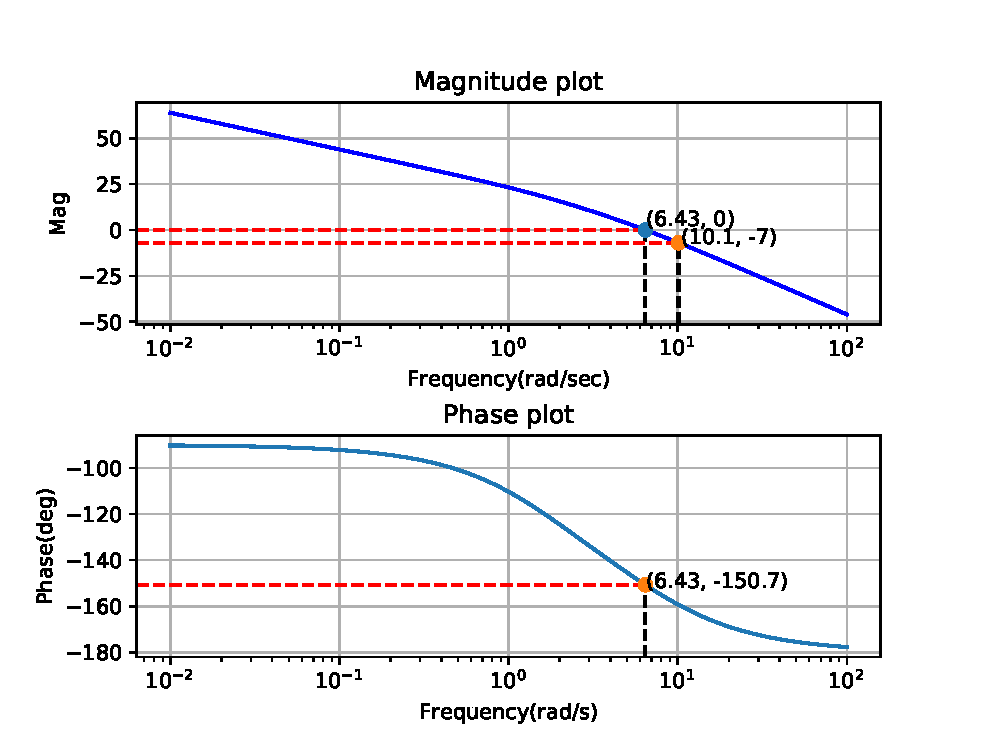
\includegraphics[width=\columnwidth]{./figs/ee18btech11047/ee18btech11047_2.eps}
\caption{1}
\label{fig:ee18btech11047_2}
\end{figure}
The phase margin is 
\begin{align}
\phi_{M} &= 180\degree-150.7\degree \implies \phi_{M} = 29.3\degree \label{eq:ee18btech11047_ph}
\end{align}
The closed-loop bandwith, $\omega_{BW}$(-3 dB frequency), equals the frequency at which the open-loop magnitude response is around -7 dB.
\begin{align}
\omega_{BW} = 10.1  rad/sec \label{eq:ee18btech11047_bw}
\end{align}
\textbf{Damping ratio:}
Substitute $\phi_{M}$ value from equation \eqref{eq:ee18btech11047_ph}
\begin{align}
\phi_{M} &= {tan}^{-1}\brak{\frac{2\zeta}{\sqrt{-2\zeta^{2}+\sqrt{1+4\zeta^{2}}}}}
\end{align}
\begin{align}
\implies \zeta &= 0.34
\end{align}
\textbf{Settling time:}
Substitute $\omega_{BW}$ value from equation\eqref{eq:ee18btech11047_bw} and $\zeta$
\begin{align}
T_{s}&= \frac{4}{\omega_{BW}\zeta}\sqrt{(1-2\zeta^2)+\sqrt{4\zeta^4-4\zeta^2+2}}
\end{align}
\begin{align}
\implies T_{s} &= 1.65 sec
\end{align}
\textbf{Peak time:}
\begin{align}
T_{p} &= \frac{\pi\zeta T_{s}}{4\sqrt{1-\zeta^2}}
\end{align}
\begin{align}
\implies T_{p} &= 0.325 sec
\end{align}
\textbf{Percent overshoot:}
\begin{align}
\% OS&=100e^{-(\frac{\zeta\pi}{\sqrt{1-\zeta^2}})}
\end{align}
\begin{align}
\implies \% OS &= 35.1 \%
\end{align}
Note that the answers will be approximate due to the dominant pole approximation.The following code generates the step response of the system.
\begin{lstlisting}
codes/ee18btech11047/ee18btech11047_3.py
\end{lstlisting}
\begin{figure}[!ht]
\centering
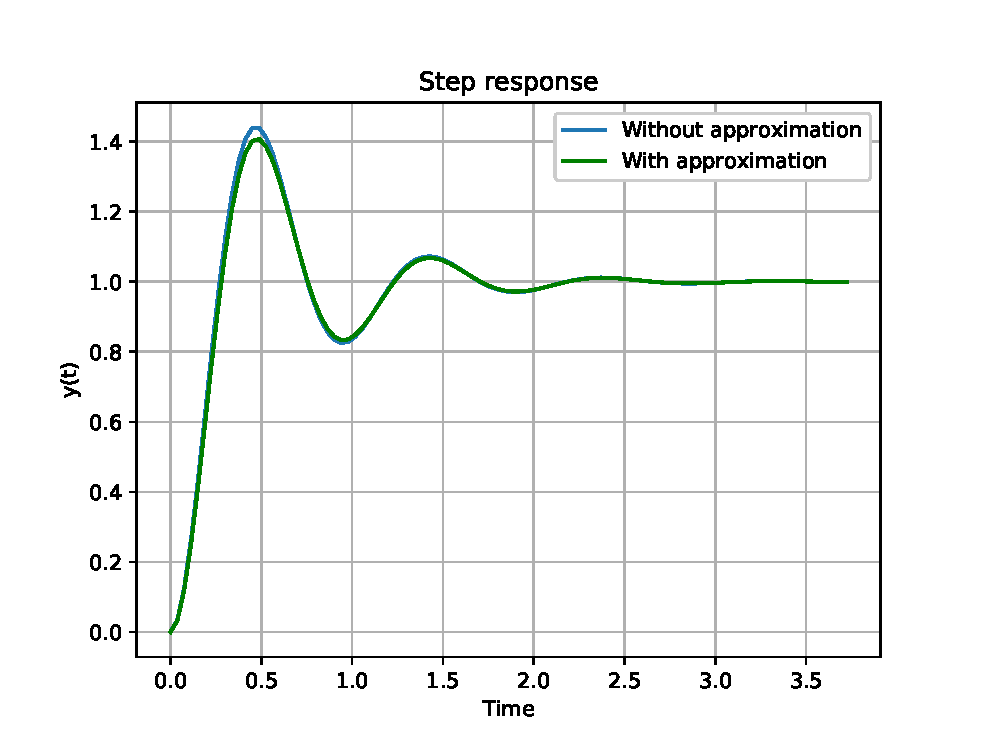
\includegraphics[width=\columnwidth]{./figs/ee18btech11047/ee18btech11047_3.eps}
\caption{2}
\label{fig:ee18btech11047_3}
\end{figure}
\item Find the approximate transfer function for the open loop transfer function
\begin{align}
G(s) &= \frac{75(1+0.2s)}{s(s^{2}+16s+100)}
\end{align}
\solution Using equation \eqref{eq:ee18btech11047_ctf}
\begin{align}
T(s) = \frac{75(1+0.2s)}{s^3 + 16s^2 + 115s +75} 
\end{align}
The following code gives the poles and zeros of the transfer function.
\begin{lstlisting}
codes/ee18btech11047/ee18btech11047_4.py
\end{lstlisting}
\begin{table}[!ht]
\centering
\input{./tables/ee18btech11047/ee18btech11047_2.tex}
\caption{}
\label{table:ee18btech11047_2}
\end{table}
The real part of the complex conjugate poles is comparable with the zero $z_{1}$ of the transfer function.So,they cancel out each other.The approximated transfer function is of first order.
\begin{align}
T_{2}(s) &= \frac{K_{2}}{(s-p_{1})}
\end{align}
\begin{align}
T(0) &= T_{2}(s)
\end{align}
\begin{align}
\implies K_{2} &= p_{1}
\end{align}
\begin{align}
T_{2}(s) &= \frac{0.72}{s+0.72}
\end{align}
\item Estimate the transient response of the obtained first order system.\\
\solution
\textbf{Time constant:}
The time constant is the time taken by the step response to rise to 63\% of it's final value.
\begin{align}
T &= \frac{1}{|pole|}
\end{align}
\begin{align}
T &= \frac{1}{0.72} = 1.388 sec
\end{align}
\textbf{Rise time:}
Rise time is the time for the waveform to go from 0.1 to 0.9 of it's final value.
\begin{align}
T_{r} &= \frac{2.2}{|pole|}
\end{align}
\begin{align}
T_{r} &= \frac{2.2}{0.72} = 3.05 sec
\end{align}
\textbf{Settling time:}
Settling time is defined as the time for the response to reach and stay within, 2\% of its final value.
\begin{align}
T_{s} &= \frac{4}{|pole|}
\end{align}
\begin{align}
T_{s} &= \frac{4}{0.72}=5.55 sec
\end{align}
The following code plots the step response of the system.
\begin{lstlisting}
codes/ee18btech11047/ee18btech11047_5.py
\end{lstlisting}
\begin{figure}[!ht]
\centering
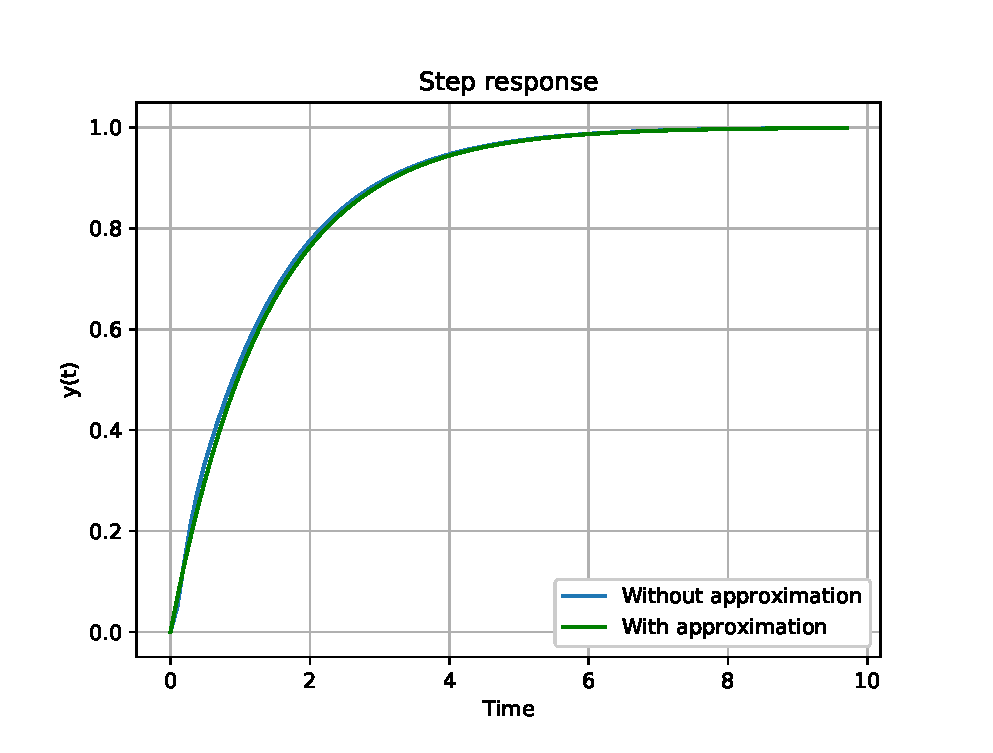
\includegraphics[width=\columnwidth]{./figs/ee18btech11047/ee18btech11047_4.eps}
\caption{}
\label{fig:ee18btech11047_4}
\end{figure}
\end{enumerate}
}
	\end{center}
\caption{}
\label{fig:ee18btech11047}
\end{figure}

\item Find the approximate transfer function for the open loop transfer function.
\begin{align}
G(s) &= \frac{50(s+3)(s+5)}{s(s+2)(s+4)(s+6)}
\end{align}
\solution Using equation\eqref{eq:ee18btech11047_ctf}
\begin{align}
T(s) &= \frac{50(s^{2}+8s+15)}{s^4+12s^3+94s^2+448s+750}
\end{align}
The following code gives the poles and zeros of the transfer function.
\begin{lstlisting}
codes/ee18btech11047/ee18btech11047_1.py
\end{lstlisting}
\begin{table}[!ht]
\centering
\begin{enumerate}[label=\thesubsection.\arabic*.,ref=\thesubsection.\theenumi]
\numberwithin{equation}{enumi}

\item Consider the following transfer functions as open-loop transfer functions in two different unity feedback(negative) systems.
\begin{align}
G(s) &= \frac{50(s+3)(s+5)}{s(s+2)(s+4)(s+6)}
\end{align}
\begin{align}
G(s) &= \frac{75(1+0.2s)}{s(s^{2}+16s+100)} 
\end{align}
Estimate transient response of these systems from their respective bode plots.\\
\solution 
\begin{enumerate}
\item  The dominant pole approximation is used to characterize higher order systems because it is difficult to characterize and analyse systems with order greater than 3.
\item Consider a transfer function.
\begin{align}
H(s) = K\frac{\alpha\beta}{(s+\alpha)(s+\beta)}
\end{align}
It has two poles $-\alpha$ and $-\beta $. If the magnitude of $\beta$ is very large compared to $\alpha$ (typically if $\frac{|\beta|}{|\alpha|}$ $>$ 5  ) we can approximate for the transfer function assuming $s$ is sufficiently small compared to $\beta$ as follows.
\begin{align}
H(s) = K_{2}\brak{\frac{1}{s+\alpha}}
\end{align}
Note that the value of $H(0)$ should be unchanged for the exact and approximate transfer functions.This is necessary to ensure that the final value of the step response is unchanged.
\begin{align}
\lim_{t\to\infty} y(t) &= \lim_{s\to 0} sY(s)
\end{align}
\begin{align}
\lim_{t\to\infty} y(t) &= \lim_{s\to 0} sU(s)H(s) = H(0)
\end{align}
In order to acheive this we adjust the gain value of the approximated transfer function by equating $H(0)$ values.
\begin{align}
\implies H(s) = K\frac{\alpha}{(s+\alpha)}
\end{align}
\item In terms of poles, the pole closer to the origin is considered as the dominating pole.As considered above,the magnitude of $\alpha$ is small therefore the time constant $\frac{1}{\alpha}$ will be high and reaches equilibrium slowly and vice versa in case of  $\beta$.Therefore,this approximation assumes that the slowest part of the system dominates the response.The faster parts of the system are ignored.
\item Complex poles along with real poles : In this case the dominant pole(s) can be determined by comparing only the real parts.If the real part of the complex conjugate poles is greater in magnitude than the real pole, the two complex conjugate poles the dominant poles.
\item If the transfer function has zeros along with poles,we have to consider the fact that pole and zero cancel out each other if their respective magnitudes are comparable.
\end{enumerate}
\item Find the closed loop transfer function of a negative unity feedback system given open loop transfer function $G(s)$ .\\
\solution 
\begin{align}
\label{eq:ee18btech11047_ctf}
T(s) &= \frac{G(s)}{1+G(s)}
\end{align}
\begin{figure}[!ht]
	\begin{center}
		\resizebox{\columnwidth}{!}{\input{./figs/ee18btech11047/ee18btech11047.tex}}
	\end{center}
\caption{}
\label{fig:ee18btech11047}
\end{figure}

\item Find the approximate transfer function for the open loop transfer function.
\begin{align}
G(s) &= \frac{50(s+3)(s+5)}{s(s+2)(s+4)(s+6)}
\end{align}
\solution Using equation\eqref{eq:ee18btech11047_ctf}
\begin{align}
T(s) &= \frac{50(s^{2}+8s+15)}{s^4+12s^3+94s^2+448s+750}
\end{align}
The following code gives the poles and zeros of the transfer function.
\begin{lstlisting}
codes/ee18btech11047/ee18btech11047_1.py
\end{lstlisting}
\begin{table}[!ht]
\centering
\input{./tables/ee18btech11047/ee18btech11047.tex}
\caption{}
\label{table:ee18btech11047}
\end{table}
The real poles \brak{p_{1},p_{2}} and zeros \brak{z_{1},z_{2}} cancel out each other as mentioned above.So, we are left with the two conjugate poles.The approximated transfer function is 
\begin{align}
T_{1}(s) &= \frac{K_{1}}{(s-p_{3})(s-p_{4})}
\end{align}
\begin{align}
T(0) &= T_{1}(0)
\end{align}
\begin{align}
\implies K_{1} &= p_{3}p_{4}
\end{align}
\begin{align}
T_{1}(s) &= \frac{47.09}{s^{2}+3.74s+47.09}
\end{align}

\item Estimate the transient response of the obtained second order system using the respective bode plot.\\
\solution The following code generates the bode plot for open loop transfer function.
\begin{lstlisting}
codes/ee18btech11047/ee18btech11047_2.py
\end{lstlisting}
\begin{figure}[!ht]
\centering
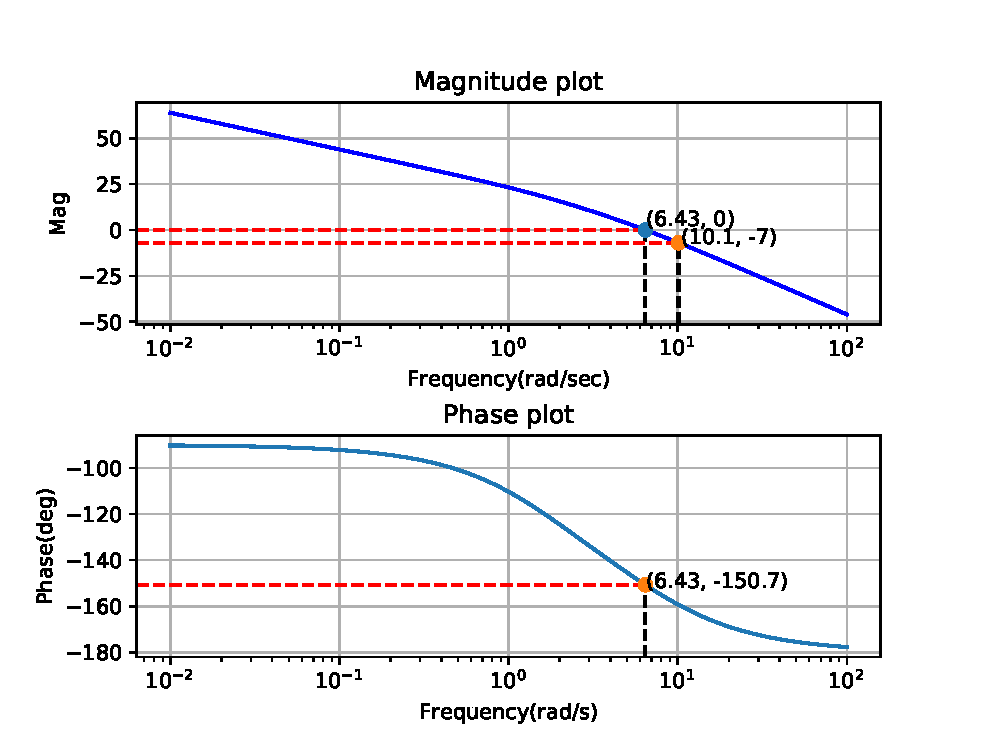
\includegraphics[width=\columnwidth]{./figs/ee18btech11047/ee18btech11047_2.eps}
\caption{1}
\label{fig:ee18btech11047_2}
\end{figure}
The phase margin is 
\begin{align}
\phi_{M} &= 180\degree-150.7\degree \implies \phi_{M} = 29.3\degree \label{eq:ee18btech11047_ph}
\end{align}
The closed-loop bandwith, $\omega_{BW}$(-3 dB frequency), equals the frequency at which the open-loop magnitude response is around -7 dB.
\begin{align}
\omega_{BW} = 10.1  rad/sec \label{eq:ee18btech11047_bw}
\end{align}
\textbf{Damping ratio:}
Substitute $\phi_{M}$ value from equation \eqref{eq:ee18btech11047_ph}
\begin{align}
\phi_{M} &= {tan}^{-1}\brak{\frac{2\zeta}{\sqrt{-2\zeta^{2}+\sqrt{1+4\zeta^{2}}}}}
\end{align}
\begin{align}
\implies \zeta &= 0.34
\end{align}
\textbf{Settling time:}
Substitute $\omega_{BW}$ value from equation\eqref{eq:ee18btech11047_bw} and $\zeta$
\begin{align}
T_{s}&= \frac{4}{\omega_{BW}\zeta}\sqrt{(1-2\zeta^2)+\sqrt{4\zeta^4-4\zeta^2+2}}
\end{align}
\begin{align}
\implies T_{s} &= 1.65 sec
\end{align}
\textbf{Peak time:}
\begin{align}
T_{p} &= \frac{\pi\zeta T_{s}}{4\sqrt{1-\zeta^2}}
\end{align}
\begin{align}
\implies T_{p} &= 0.325 sec
\end{align}
\textbf{Percent overshoot:}
\begin{align}
\% OS&=100e^{-(\frac{\zeta\pi}{\sqrt{1-\zeta^2}})}
\end{align}
\begin{align}
\implies \% OS &= 35.1 \%
\end{align}
Note that the answers will be approximate due to the dominant pole approximation.The following code generates the step response of the system.
\begin{lstlisting}
codes/ee18btech11047/ee18btech11047_3.py
\end{lstlisting}
\begin{figure}[!ht]
\centering
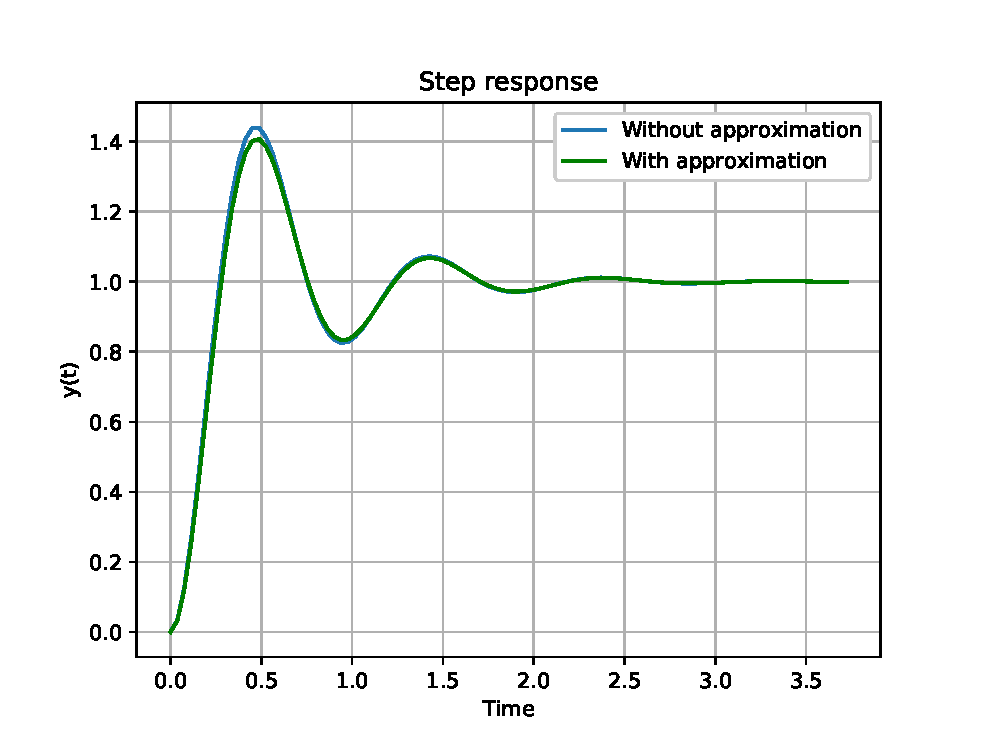
\includegraphics[width=\columnwidth]{./figs/ee18btech11047/ee18btech11047_3.eps}
\caption{2}
\label{fig:ee18btech11047_3}
\end{figure}
\item Find the approximate transfer function for the open loop transfer function
\begin{align}
G(s) &= \frac{75(1+0.2s)}{s(s^{2}+16s+100)}
\end{align}
\solution Using equation \eqref{eq:ee18btech11047_ctf}
\begin{align}
T(s) = \frac{75(1+0.2s)}{s^3 + 16s^2 + 115s +75} 
\end{align}
The following code gives the poles and zeros of the transfer function.
\begin{lstlisting}
codes/ee18btech11047/ee18btech11047_4.py
\end{lstlisting}
\begin{table}[!ht]
\centering
\input{./tables/ee18btech11047/ee18btech11047_2.tex}
\caption{}
\label{table:ee18btech11047_2}
\end{table}
The real part of the complex conjugate poles is comparable with the zero $z_{1}$ of the transfer function.So,they cancel out each other.The approximated transfer function is of first order.
\begin{align}
T_{2}(s) &= \frac{K_{2}}{(s-p_{1})}
\end{align}
\begin{align}
T(0) &= T_{2}(s)
\end{align}
\begin{align}
\implies K_{2} &= p_{1}
\end{align}
\begin{align}
T_{2}(s) &= \frac{0.72}{s+0.72}
\end{align}
\item Estimate the transient response of the obtained first order system.\\
\solution
\textbf{Time constant:}
The time constant is the time taken by the step response to rise to 63\% of it's final value.
\begin{align}
T &= \frac{1}{|pole|}
\end{align}
\begin{align}
T &= \frac{1}{0.72} = 1.388 sec
\end{align}
\textbf{Rise time:}
Rise time is the time for the waveform to go from 0.1 to 0.9 of it's final value.
\begin{align}
T_{r} &= \frac{2.2}{|pole|}
\end{align}
\begin{align}
T_{r} &= \frac{2.2}{0.72} = 3.05 sec
\end{align}
\textbf{Settling time:}
Settling time is defined as the time for the response to reach and stay within, 2\% of its final value.
\begin{align}
T_{s} &= \frac{4}{|pole|}
\end{align}
\begin{align}
T_{s} &= \frac{4}{0.72}=5.55 sec
\end{align}
The following code plots the step response of the system.
\begin{lstlisting}
codes/ee18btech11047/ee18btech11047_5.py
\end{lstlisting}
\begin{figure}[!ht]
\centering
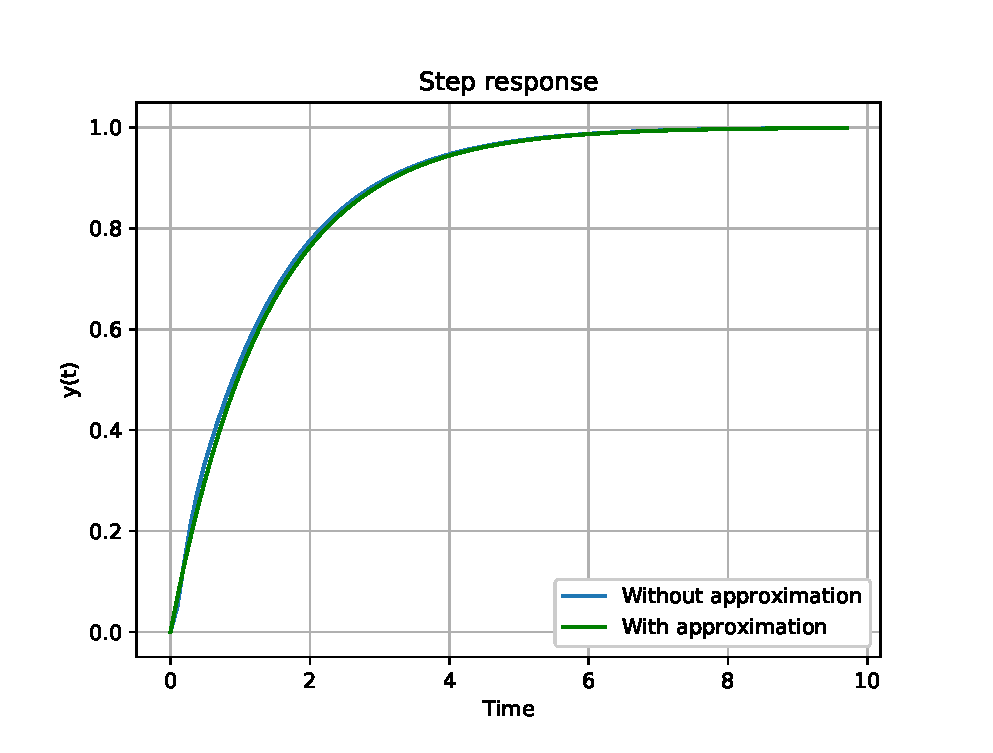
\includegraphics[width=\columnwidth]{./figs/ee18btech11047/ee18btech11047_4.eps}
\caption{}
\label{fig:ee18btech11047_4}
\end{figure}
\end{enumerate}

\caption{}
\label{table:ee18btech11047}
\end{table}
The real poles \brak{p_{1},p_{2}} and zeros \brak{z_{1},z_{2}} cancel out each other as mentioned above.So, we are left with the two conjugate poles.The approximated transfer function is 
\begin{align}
T_{1}(s) &= \frac{K_{1}}{(s-p_{3})(s-p_{4})}
\end{align}
\begin{align}
T(0) &= T_{1}(0)
\end{align}
\begin{align}
\implies K_{1} &= p_{3}p_{4}
\end{align}
\begin{align}
T_{1}(s) &= \frac{47.09}{s^{2}+3.74s+47.09}
\end{align}

\item Estimate the transient response of the obtained second order system using the respective bode plot.\\
\solution The following code generates the bode plot for open loop transfer function.
\begin{lstlisting}
codes/ee18btech11047/ee18btech11047_2.py
\end{lstlisting}
\begin{figure}[!ht]
\centering
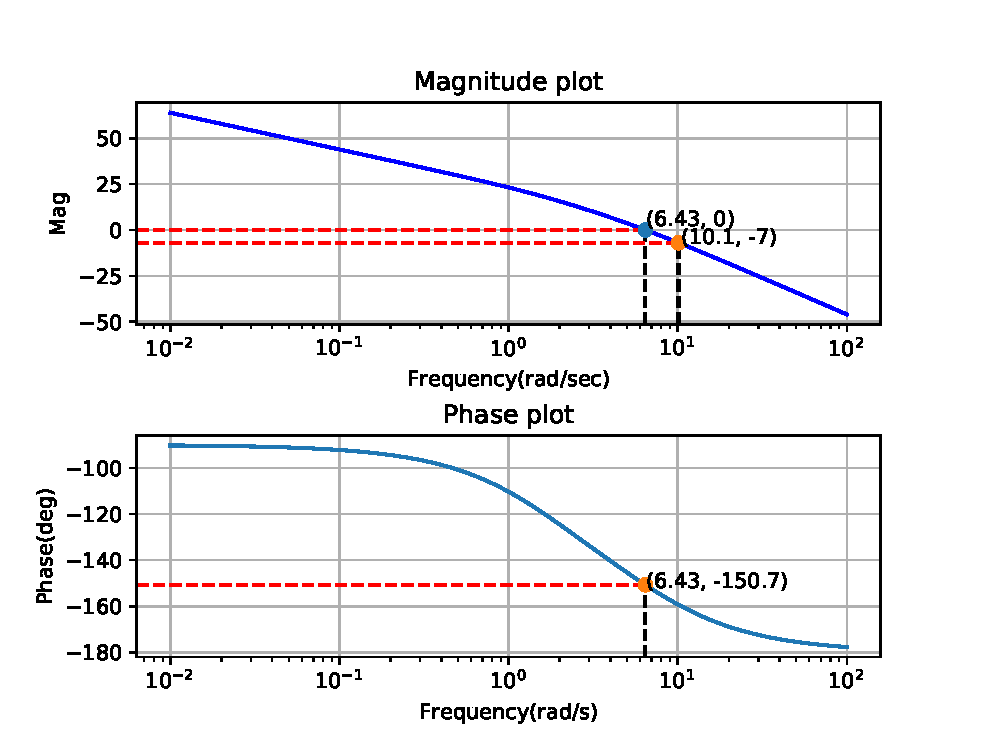
\includegraphics[width=\columnwidth]{./figs/ee18btech11047/ee18btech11047_2.eps}
\caption{1}
\label{fig:ee18btech11047_2}
\end{figure}
The phase margin is 
\begin{align}
\phi_{M} &= 180\degree-150.7\degree \implies \phi_{M} = 29.3\degree \label{eq:ee18btech11047_ph}
\end{align}
The closed-loop bandwith, $\omega_{BW}$(-3 dB frequency), equals the frequency at which the open-loop magnitude response is around -7 dB.
\begin{align}
\omega_{BW} = 10.1  rad/sec \label{eq:ee18btech11047_bw}
\end{align}
\textbf{Damping ratio:}
Substitute $\phi_{M}$ value from equation \eqref{eq:ee18btech11047_ph}
\begin{align}
\phi_{M} &= {tan}^{-1}\brak{\frac{2\zeta}{\sqrt{-2\zeta^{2}+\sqrt{1+4\zeta^{2}}}}}
\end{align}
\begin{align}
\implies \zeta &= 0.34
\end{align}
\textbf{Settling time:}
Substitute $\omega_{BW}$ value from equation\eqref{eq:ee18btech11047_bw} and $\zeta$
\begin{align}
T_{s}&= \frac{4}{\omega_{BW}\zeta}\sqrt{(1-2\zeta^2)+\sqrt{4\zeta^4-4\zeta^2+2}}
\end{align}
\begin{align}
\implies T_{s} &= 1.65 sec
\end{align}
\textbf{Peak time:}
\begin{align}
T_{p} &= \frac{\pi\zeta T_{s}}{4\sqrt{1-\zeta^2}}
\end{align}
\begin{align}
\implies T_{p} &= 0.325 sec
\end{align}
\textbf{Percent overshoot:}
\begin{align}
\% OS&=100e^{-(\frac{\zeta\pi}{\sqrt{1-\zeta^2}})}
\end{align}
\begin{align}
\implies \% OS &= 35.1 \%
\end{align}
Note that the answers will be approximate due to the dominant pole approximation.The following code generates the step response of the system.
\begin{lstlisting}
codes/ee18btech11047/ee18btech11047_3.py
\end{lstlisting}
\begin{figure}[!ht]
\centering
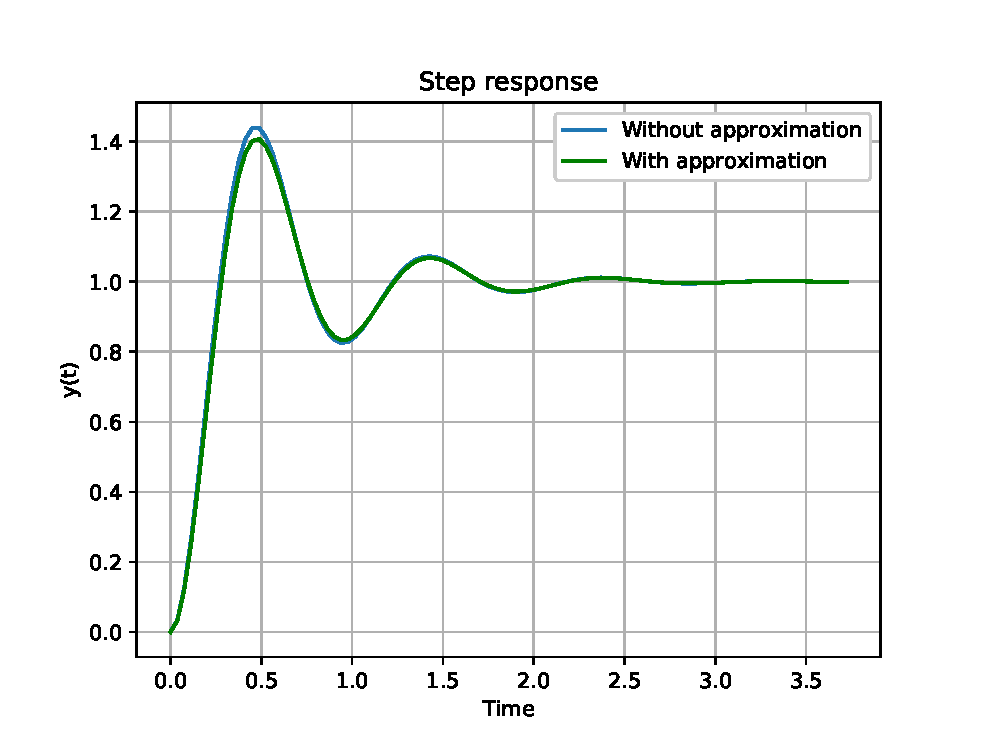
\includegraphics[width=\columnwidth]{./figs/ee18btech11047/ee18btech11047_3.eps}
\caption{2}
\label{fig:ee18btech11047_3}
\end{figure}
\item Find the approximate transfer function for the open loop transfer function
\begin{align}
G(s) &= \frac{75(1+0.2s)}{s(s^{2}+16s+100)}
\end{align}
\solution Using equation \eqref{eq:ee18btech11047_ctf}
\begin{align}
T(s) = \frac{75(1+0.2s)}{s^3 + 16s^2 + 115s +75} 
\end{align}
The following code gives the poles and zeros of the transfer function.
\begin{lstlisting}
codes/ee18btech11047/ee18btech11047_4.py
\end{lstlisting}
\begin{table}[!ht]
\centering
%%%%%%%%%%%%%%%%%%%%%%%%%%%%%%%%%%%%%%%%%%%%%%%%%%%%%%%%%%%%%%%%%%%%%%
%%                                                                  %%
%%  This is the header of a LaTeX2e file exported from Gnumeric.    %%
%%                                                                  %%
%%  This file can be compiled as it stands or included in another   %%
%%  LaTeX document. The table is based on the longtable package so  %%
%%  the longtable options (headers, footers...) can be set in the   %%
%%  preamble section below (see PRAMBLE).                           %%
%%                                                                  %%
%%  To include the file in another, the following two lines must be %%
%%  in the including file:                                          %%
%%        \def\inputGnumericTable{}                                 %%
%%  at the beginning of the file and:                               %%
%%        \input{name-of-this-file.tex}                             %%
%%  where the table is to be placed. Note also that the including   %%
%%  file must use the following packages for the table to be        %%
%%  rendered correctly:                                             %%
%%    \usepackage[latin1]{inputenc}                                 %%
%%    \usepackage{color}                                            %%
%%    \usepackage{array}                                            %%
%%    \usepackage{longtable}                                        %%
%%    \usepackage{calc}                                             %%
%%    \usepackage{multirow}                                         %%
%%    \usepackage{hhline}                                           %%
%%    \usepackage{ifthen}                                           %%
%%  optionally (for landscape tables embedded in another document): %%
%%    \usepackage{lscape}                                           %%
%%                                                                  %%
%%%%%%%%%%%%%%%%%%%%%%%%%%%%%%%%%%%%%%%%%%%%%%%%%%%%%%%%%%%%%%%%%%%%%%



%%  This section checks if we are begin input into another file or  %%
%%  the file will be compiled alone. First use a macro taken from   %%
%%  the TeXbook ex 7.7 (suggestion of Han-Wen Nienhuys).            %%
\def\ifundefined#1{\expandafter\ifx\csname#1\endcsname\relax}


%%  Check for the \def token for inputed files. If it is not        %%
%%  defined, the file will be processed as a standalone and the     %%
%%  preamble will be used.                                          %%
\ifundefined{inputGnumericTable}

%%  We must be able to close or not the document at the end.        %%
	\def\gnumericTableEnd{\end{document}}


%%%%%%%%%%%%%%%%%%%%%%%%%%%%%%%%%%%%%%%%%%%%%%%%%%%%%%%%%%%%%%%%%%%%%%
%%                                                                  %%
%%  This is the PREAMBLE. Change these values to get the right      %%
%%  paper size and other niceties.                                  %%
%%                                                                  %%
%%%%%%%%%%%%%%%%%%%%%%%%%%%%%%%%%%%%%%%%%%%%%%%%%%%%%%%%%%%%%%%%%%%%%%

	\documentclass[12pt%
			  %,landscape%
                    ]{report}
       \usepackage[latin1]{inputenc}
       \usepackage{fullpage}
       \usepackage{color}
       \usepackage{array}
       \usepackage{longtable}
       \usepackage{calc}
       \usepackage{multirow}
       \usepackage{hhline}
       \usepackage{ifthen}

	\begin{document}


%%  End of the preamble for the standalone. The next section is for %%
%%  documents which are included into other LaTeX2e files.          %%
\else

%%  We are not a stand alone document. For a regular table, we will %%
%%  have no preamble and only define the closing to mean nothing.   %%
    \def\gnumericTableEnd{}

%%  If we want landscape mode in an embedded document, comment out  %%
%%  the line above and uncomment the two below. The table will      %%
%%  begin on a new page and run in landscape mode.                  %%
%       \def\gnumericTableEnd{\end{landscape}}
%       \begin{landscape}


%%  End of the else clause for this file being \input.              %%
\fi

%%%%%%%%%%%%%%%%%%%%%%%%%%%%%%%%%%%%%%%%%%%%%%%%%%%%%%%%%%%%%%%%%%%%%%
%%                                                                  %%
%%  The rest is the gnumeric table, except for the closing          %%
%%  statement. Changes below will alter the table's appearance.     %%
%%                                                                  %%
%%%%%%%%%%%%%%%%%%%%%%%%%%%%%%%%%%%%%%%%%%%%%%%%%%%%%%%%%%%%%%%%%%%%%%

\providecommand{\gnumericmathit}[1]{#1} 
%%  Uncomment the next line if you would like your numbers to be in %%
%%  italics if they are italizised in the gnumeric table.           %%
%\renewcommand{\gnumericmathit}[1]{\mathit{#1}}
\providecommand{\gnumericPB}[1]%
{\let\gnumericTemp=\\#1\let\\=\gnumericTemp\hspace{0pt}}
 \ifundefined{gnumericTableWidthDefined}
        \newlength{\gnumericTableWidth}
        \newlength{\gnumericTableWidthComplete}
        \newlength{\gnumericMultiRowLength}
        \global\def\gnumericTableWidthDefined{}
 \fi
%% The following setting protects this code from babel shorthands.  %%
 \ifthenelse{\isundefined{\languageshorthands}}{}{\languageshorthands{english}}
%%  The default table format retains the relative column widths of  %%
%%  gnumeric. They can easily be changed to c, r or l. In that case %%
%%  you may want to comment out the next line and uncomment the one %%
%%  thereafter                                                      %%
\providecommand\gnumbox{\makebox[0pt]}
%%\providecommand\gnumbox[1][]{\makebox}

%% to adjust positions in multirow situations                       %%
\setlength{\bigstrutjot}{\jot}
\setlength{\extrarowheight}{\doublerulesep}

%%  The \setlongtables command keeps column widths the same across  %%
%%  pages. Simply comment out next line for varying column widths.  %%
\setlongtables

\setlength\gnumericTableWidth{%
	53pt+%
	93pt+%
0pt}
\def\gumericNumCols{2}
\setlength\gnumericTableWidthComplete{\gnumericTableWidth+%
         \tabcolsep*\gumericNumCols*2+\arrayrulewidth*\gumericNumCols}
\ifthenelse{\lengthtest{\gnumericTableWidthComplete > \linewidth}}%
         {\def\gnumericScale{\ratio{\linewidth-%
                        \tabcolsep*\gumericNumCols*2-%
                        \arrayrulewidth*\gumericNumCols}%
{\gnumericTableWidth}}}%
{\def\gnumericScale{1}}

%%%%%%%%%%%%%%%%%%%%%%%%%%%%%%%%%%%%%%%%%%%%%%%%%%%%%%%%%%%%%%%%%%%%%%
%%                                                                  %%
%% The following are the widths of the various columns. We are      %%
%% defining them here because then they are easier to change.       %%
%% Depending on the cell formats we may use them more than once.    %%
%%                                                                  %%
%%%%%%%%%%%%%%%%%%%%%%%%%%%%%%%%%%%%%%%%%%%%%%%%%%%%%%%%%%%%%%%%%%%%%%

\ifthenelse{\isundefined{\gnumericColA}}{\newlength{\gnumericColA}}{}\settowidth{\gnumericColA}{\begin{tabular}{@{}p{90pt*\gnumericScale}@{}}x\end{tabular}}
\ifthenelse{\isundefined{\gnumericColB}}{\newlength{\gnumericColB}}{}\settowidth{\gnumericColB}{\begin{tabular}{@{}p{53pt*\gnumericScale}@{}}x\end{tabular}}

\begin{tabular}[c]{%
	b{\gnumericColA}%
	b{\gnumericColB}%
	}

%%%%%%%%%%%%%%%%%%%%%%%%%%%%%%%%%%%%%%%%%%%%%%%%%%%%%%%%%%%%%%%%%%%%%%
%%  The longtable options. (Caption, headers... see Goosens, p.124) %%
%	\caption{The Table Caption.}             \\	%
% \hline	% Across the top of the table.
%%  The rest of these options are table rows which are placed on    %%
%%  the first, last or every page. Use \multicolumn if you want.    %%

%%  Header for the first page.                                      %%
%	\multicolumn{2}{c}{The First Header} \\ \hline 
%	\multicolumn{1}{c}{colTag}	%Column 1
%	&\multicolumn{1}{c}{colTag}	\\ \hline %Last column
%	\endfirsthead

%%  The running header definition.                                  %%
%	\hline
%	\multicolumn{2}{l}{\ldots\small\slshape continued} \\ \hline
%	\multicolumn{1}{c}{colTag}	%Column 1
%	&\multicolumn{1}{c}{colTag}	\\ \hline %Last column
%	\endhead

%%  The running footer definition.                                  %%
%	\hline
%	\multicolumn{2}{r}{\small\slshape continued\ldots} \\
%	\endfoot

%%  The ending footer definition.                                   %%
%	\multicolumn{2}{c}{That's all folks} \\ \hline 
%	\endlastfoot
%%%%%%%%%%%%%%%%%%%%%%%%%%%%%%%%%%%%%%%%%%%%%%%%%%%%%%%%%%%%%%%%%%%%%%

\hhline{|-|-}
	 \multicolumn{1}{|p{\gnumericColA}|}%
	{\gnumericPB{\centering}\gnumbox{\textbf{Poles}}}
	&\multicolumn{1}{p{\gnumericColB}|}%
	{\gnumericPB{\centering}\gnumbox{\textbf{Zeros}}}
\\
\hhline{|--|}
	 \multicolumn{1}{|p{\gnumericColA}|}%
	{\gnumericPB{\centering}\gnumbox{$p_{1}=-0.72$}}
	&\multicolumn{1}{p{\gnumericColB}|}%
	{$z_{1}=-5$}
\\
\hhline{|--|}
	 \multicolumn{1}{|p{\gnumericColA}|}%
	{\gnumericPB{\centering}\gnumbox{$p_{2}=-7.64+6.75j$}}
	&\multicolumn{1}{p{\gnumericColB}|}%
	{}
\\
\hhline{|--|}
	 \multicolumn{1}{|p{\gnumericColA}|}%
	{\gnumericPB{\centering}\gnumbox{$p_{3}=-7.63-6.75j$}}
	&\multicolumn{1}{p{\gnumericColB}|}%
	{}
\\
\hhline{|-|-|}
\end{tabular}

\ifthenelse{\isundefined{\languageshorthands}}{}{\languageshorthands{\languagename}}
\gnumericTableEnd

\caption{}
\label{table:ee18btech11047_2}
\end{table}
The real part of the complex conjugate poles is comparable with the zero $z_{1}$ of the transfer function.So,they cancel out each other.The approximated transfer function is of first order.
\begin{align}
T_{2}(s) &= \frac{K_{2}}{(s-p_{1})}
\end{align}
\begin{align}
T(0) &= T_{2}(s)
\end{align}
\begin{align}
\implies K_{2} &= p_{1}
\end{align}
\begin{align}
T_{2}(s) &= \frac{0.72}{s+0.72}
\end{align}
\item Estimate the transient response of the obtained first order system.\\
\solution
\textbf{Time constant:}
The time constant is the time taken by the step response to rise to 63\% of it's final value.
\begin{align}
T &= \frac{1}{|pole|}
\end{align}
\begin{align}
T &= \frac{1}{0.72} = 1.388 sec
\end{align}
\textbf{Rise time:}
Rise time is the time for the waveform to go from 0.1 to 0.9 of it's final value.
\begin{align}
T_{r} &= \frac{2.2}{|pole|}
\end{align}
\begin{align}
T_{r} &= \frac{2.2}{0.72} = 3.05 sec
\end{align}
\textbf{Settling time:}
Settling time is defined as the time for the response to reach and stay within, 2\% of its final value.
\begin{align}
T_{s} &= \frac{4}{|pole|}
\end{align}
\begin{align}
T_{s} &= \frac{4}{0.72}=5.55 sec
\end{align}
The following code plots the step response of the system.
\begin{lstlisting}
codes/ee18btech11047/ee18btech11047_5.py
\end{lstlisting}
\begin{figure}[!ht]
\centering
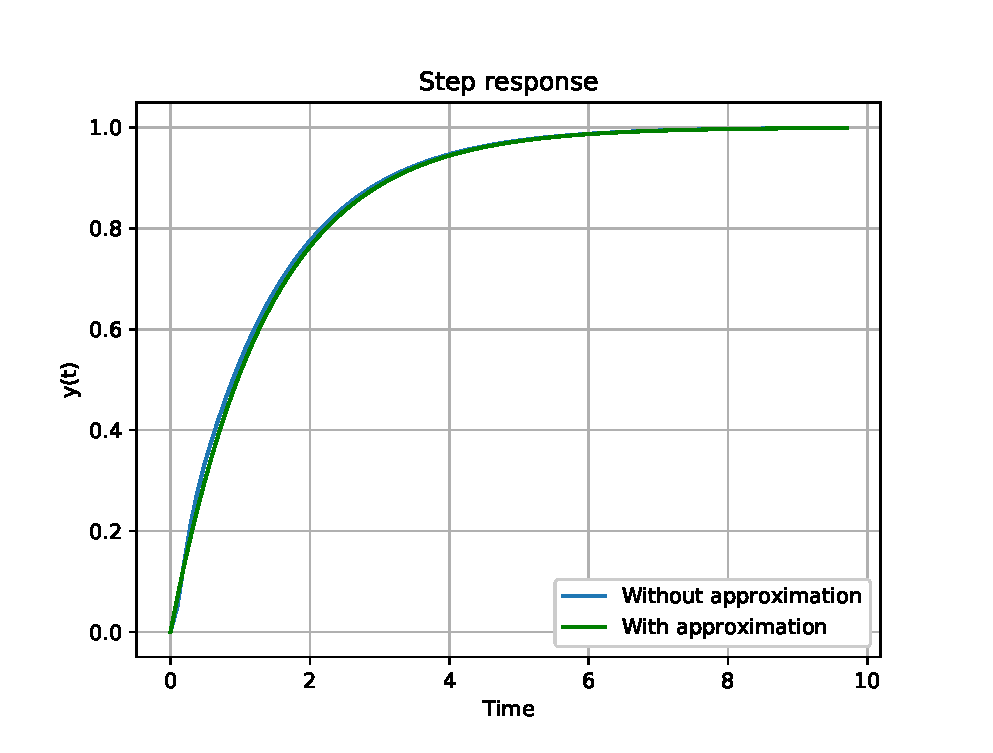
\includegraphics[width=\columnwidth]{./figs/ee18btech11047/ee18btech11047_4.eps}
\caption{}
\label{fig:ee18btech11047_4}
\end{figure}
\end{enumerate}
}
	\end{center}
\caption{}
\label{fig:ee18btech11047}
\end{figure}

\item Find the approximate transfer function for the open loop transfer function.
\begin{align}
G(s) &= \frac{50(s+3)(s+5)}{s(s+2)(s+4)(s+6)}
\end{align}
\solution Using equation\eqref{eq:ee18btech11047_ctf}
\begin{align}
T(s) &= \frac{50(s^{2}+8s+15)}{s^4+12s^3+94s^2+448s+750}
\end{align}
The following code gives the poles and zeros of the transfer function.
\begin{lstlisting}
codes/ee18btech11047/ee18btech11047_1.py
\end{lstlisting}
\begin{table}[!ht]
\centering
\begin{enumerate}[label=\thesubsection.\arabic*.,ref=\thesubsection.\theenumi]
\numberwithin{equation}{enumi}

\item Consider the following transfer functions as open-loop transfer functions in two different unity feedback(negative) systems.
\begin{align}
G(s) &= \frac{50(s+3)(s+5)}{s(s+2)(s+4)(s+6)}
\end{align}
\begin{align}
G(s) &= \frac{75(1+0.2s)}{s(s^{2}+16s+100)} 
\end{align}
Estimate transient response of these systems from their respective bode plots.\\
\solution 
\begin{enumerate}
\item  The dominant pole approximation is used to characterize higher order systems because it is difficult to characterize and analyse systems with order greater than 3.
\item Consider a transfer function.
\begin{align}
H(s) = K\frac{\alpha\beta}{(s+\alpha)(s+\beta)}
\end{align}
It has two poles $-\alpha$ and $-\beta $. If the magnitude of $\beta$ is very large compared to $\alpha$ (typically if $\frac{|\beta|}{|\alpha|}$ $>$ 5  ) we can approximate for the transfer function assuming $s$ is sufficiently small compared to $\beta$ as follows.
\begin{align}
H(s) = K_{2}\brak{\frac{1}{s+\alpha}}
\end{align}
Note that the value of $H(0)$ should be unchanged for the exact and approximate transfer functions.This is necessary to ensure that the final value of the step response is unchanged.
\begin{align}
\lim_{t\to\infty} y(t) &= \lim_{s\to 0} sY(s)
\end{align}
\begin{align}
\lim_{t\to\infty} y(t) &= \lim_{s\to 0} sU(s)H(s) = H(0)
\end{align}
In order to acheive this we adjust the gain value of the approximated transfer function by equating $H(0)$ values.
\begin{align}
\implies H(s) = K\frac{\alpha}{(s+\alpha)}
\end{align}
\item In terms of poles, the pole closer to the origin is considered as the dominating pole.As considered above,the magnitude of $\alpha$ is small therefore the time constant $\frac{1}{\alpha}$ will be high and reaches equilibrium slowly and vice versa in case of  $\beta$.Therefore,this approximation assumes that the slowest part of the system dominates the response.The faster parts of the system are ignored.
\item Complex poles along with real poles : In this case the dominant pole(s) can be determined by comparing only the real parts.If the real part of the complex conjugate poles is greater in magnitude than the real pole, the two complex conjugate poles the dominant poles.
\item If the transfer function has zeros along with poles,we have to consider the fact that pole and zero cancel out each other if their respective magnitudes are comparable.
\end{enumerate}
\item Find the closed loop transfer function of a negative unity feedback system given open loop transfer function $G(s)$ .\\
\solution 
\begin{align}
\label{eq:ee18btech11047_ctf}
T(s) &= \frac{G(s)}{1+G(s)}
\end{align}
\begin{figure}[!ht]
	\begin{center}
		\resizebox{\columnwidth}{!}{\begin{enumerate}[label=\thesubsection.\arabic*.,ref=\thesubsection.\theenumi]
\numberwithin{equation}{enumi}

\item Consider the following transfer functions as open-loop transfer functions in two different unity feedback(negative) systems.
\begin{align}
G(s) &= \frac{50(s+3)(s+5)}{s(s+2)(s+4)(s+6)}
\end{align}
\begin{align}
G(s) &= \frac{75(1+0.2s)}{s(s^{2}+16s+100)} 
\end{align}
Estimate transient response of these systems from their respective bode plots.\\
\solution 
\begin{enumerate}
\item  The dominant pole approximation is used to characterize higher order systems because it is difficult to characterize and analyse systems with order greater than 3.
\item Consider a transfer function.
\begin{align}
H(s) = K\frac{\alpha\beta}{(s+\alpha)(s+\beta)}
\end{align}
It has two poles $-\alpha$ and $-\beta $. If the magnitude of $\beta$ is very large compared to $\alpha$ (typically if $\frac{|\beta|}{|\alpha|}$ $>$ 5  ) we can approximate for the transfer function assuming $s$ is sufficiently small compared to $\beta$ as follows.
\begin{align}
H(s) = K_{2}\brak{\frac{1}{s+\alpha}}
\end{align}
Note that the value of $H(0)$ should be unchanged for the exact and approximate transfer functions.This is necessary to ensure that the final value of the step response is unchanged.
\begin{align}
\lim_{t\to\infty} y(t) &= \lim_{s\to 0} sY(s)
\end{align}
\begin{align}
\lim_{t\to\infty} y(t) &= \lim_{s\to 0} sU(s)H(s) = H(0)
\end{align}
In order to acheive this we adjust the gain value of the approximated transfer function by equating $H(0)$ values.
\begin{align}
\implies H(s) = K\frac{\alpha}{(s+\alpha)}
\end{align}
\item In terms of poles, the pole closer to the origin is considered as the dominating pole.As considered above,the magnitude of $\alpha$ is small therefore the time constant $\frac{1}{\alpha}$ will be high and reaches equilibrium slowly and vice versa in case of  $\beta$.Therefore,this approximation assumes that the slowest part of the system dominates the response.The faster parts of the system are ignored.
\item Complex poles along with real poles : In this case the dominant pole(s) can be determined by comparing only the real parts.If the real part of the complex conjugate poles is greater in magnitude than the real pole, the two complex conjugate poles the dominant poles.
\item If the transfer function has zeros along with poles,we have to consider the fact that pole and zero cancel out each other if their respective magnitudes are comparable.
\end{enumerate}
\item Find the closed loop transfer function of a negative unity feedback system given open loop transfer function $G(s)$ .\\
\solution 
\begin{align}
\label{eq:ee18btech11047_ctf}
T(s) &= \frac{G(s)}{1+G(s)}
\end{align}
\begin{figure}[!ht]
	\begin{center}
		\resizebox{\columnwidth}{!}{\input{./figs/ee18btech11047/ee18btech11047.tex}}
	\end{center}
\caption{}
\label{fig:ee18btech11047}
\end{figure}

\item Find the approximate transfer function for the open loop transfer function.
\begin{align}
G(s) &= \frac{50(s+3)(s+5)}{s(s+2)(s+4)(s+6)}
\end{align}
\solution Using equation\eqref{eq:ee18btech11047_ctf}
\begin{align}
T(s) &= \frac{50(s^{2}+8s+15)}{s^4+12s^3+94s^2+448s+750}
\end{align}
The following code gives the poles and zeros of the transfer function.
\begin{lstlisting}
codes/ee18btech11047/ee18btech11047_1.py
\end{lstlisting}
\begin{table}[!ht]
\centering
\input{./tables/ee18btech11047/ee18btech11047.tex}
\caption{}
\label{table:ee18btech11047}
\end{table}
The real poles \brak{p_{1},p_{2}} and zeros \brak{z_{1},z_{2}} cancel out each other as mentioned above.So, we are left with the two conjugate poles.The approximated transfer function is 
\begin{align}
T_{1}(s) &= \frac{K_{1}}{(s-p_{3})(s-p_{4})}
\end{align}
\begin{align}
T(0) &= T_{1}(0)
\end{align}
\begin{align}
\implies K_{1} &= p_{3}p_{4}
\end{align}
\begin{align}
T_{1}(s) &= \frac{47.09}{s^{2}+3.74s+47.09}
\end{align}

\item Estimate the transient response of the obtained second order system using the respective bode plot.\\
\solution The following code generates the bode plot for open loop transfer function.
\begin{lstlisting}
codes/ee18btech11047/ee18btech11047_2.py
\end{lstlisting}
\begin{figure}[!ht]
\centering
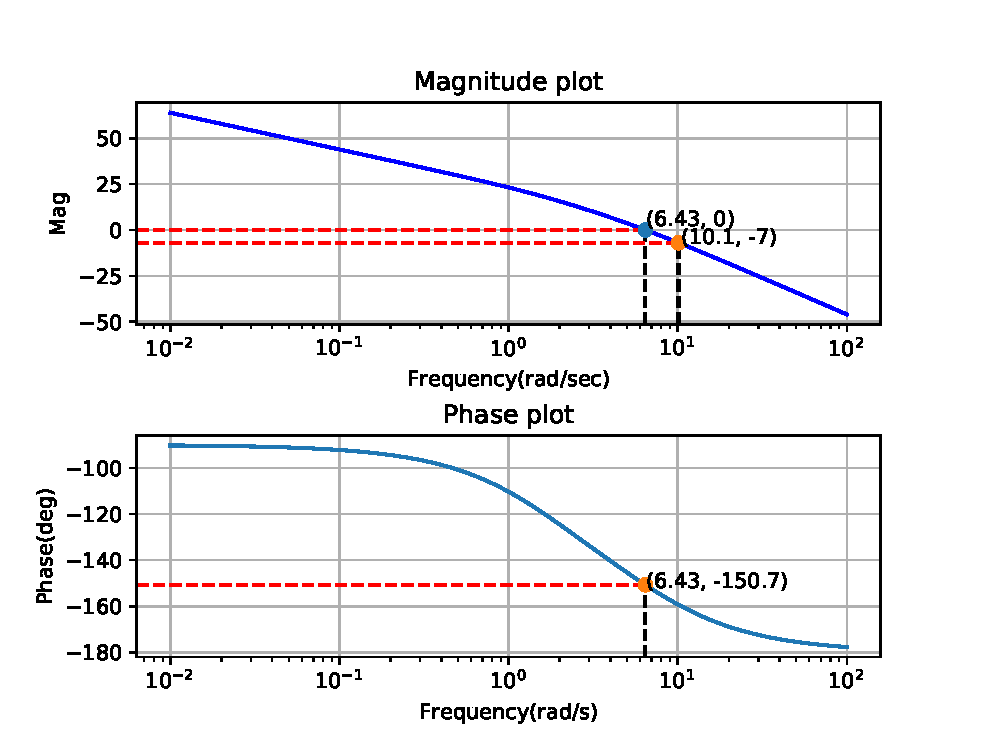
\includegraphics[width=\columnwidth]{./figs/ee18btech11047/ee18btech11047_2.eps}
\caption{1}
\label{fig:ee18btech11047_2}
\end{figure}
The phase margin is 
\begin{align}
\phi_{M} &= 180\degree-150.7\degree \implies \phi_{M} = 29.3\degree \label{eq:ee18btech11047_ph}
\end{align}
The closed-loop bandwith, $\omega_{BW}$(-3 dB frequency), equals the frequency at which the open-loop magnitude response is around -7 dB.
\begin{align}
\omega_{BW} = 10.1  rad/sec \label{eq:ee18btech11047_bw}
\end{align}
\textbf{Damping ratio:}
Substitute $\phi_{M}$ value from equation \eqref{eq:ee18btech11047_ph}
\begin{align}
\phi_{M} &= {tan}^{-1}\brak{\frac{2\zeta}{\sqrt{-2\zeta^{2}+\sqrt{1+4\zeta^{2}}}}}
\end{align}
\begin{align}
\implies \zeta &= 0.34
\end{align}
\textbf{Settling time:}
Substitute $\omega_{BW}$ value from equation\eqref{eq:ee18btech11047_bw} and $\zeta$
\begin{align}
T_{s}&= \frac{4}{\omega_{BW}\zeta}\sqrt{(1-2\zeta^2)+\sqrt{4\zeta^4-4\zeta^2+2}}
\end{align}
\begin{align}
\implies T_{s} &= 1.65 sec
\end{align}
\textbf{Peak time:}
\begin{align}
T_{p} &= \frac{\pi\zeta T_{s}}{4\sqrt{1-\zeta^2}}
\end{align}
\begin{align}
\implies T_{p} &= 0.325 sec
\end{align}
\textbf{Percent overshoot:}
\begin{align}
\% OS&=100e^{-(\frac{\zeta\pi}{\sqrt{1-\zeta^2}})}
\end{align}
\begin{align}
\implies \% OS &= 35.1 \%
\end{align}
Note that the answers will be approximate due to the dominant pole approximation.The following code generates the step response of the system.
\begin{lstlisting}
codes/ee18btech11047/ee18btech11047_3.py
\end{lstlisting}
\begin{figure}[!ht]
\centering
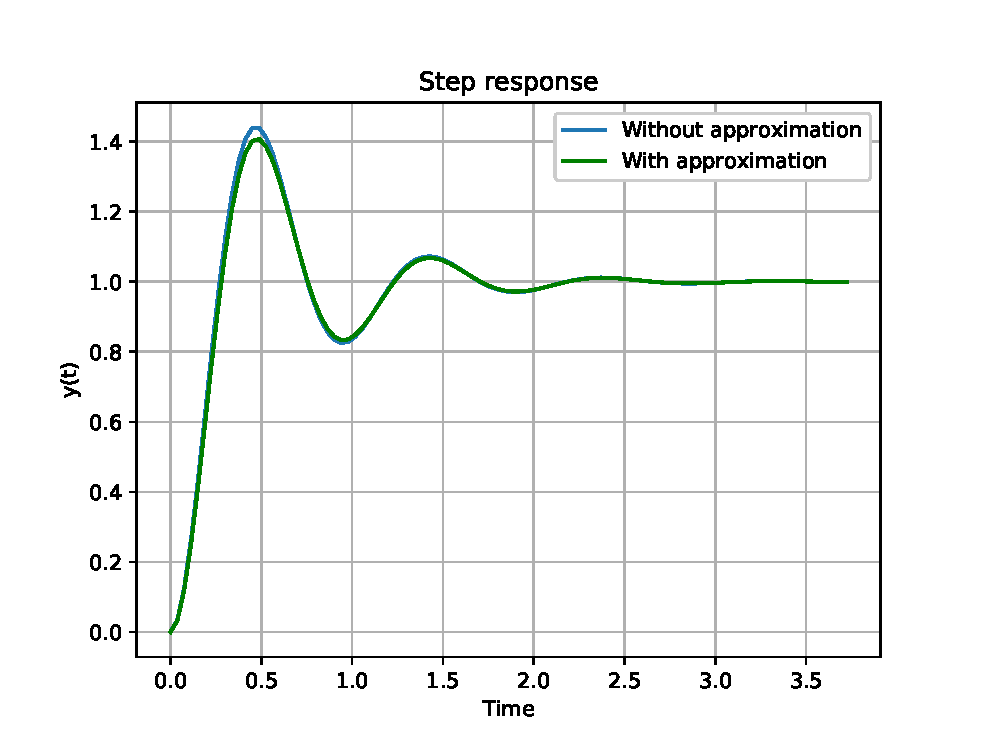
\includegraphics[width=\columnwidth]{./figs/ee18btech11047/ee18btech11047_3.eps}
\caption{2}
\label{fig:ee18btech11047_3}
\end{figure}
\item Find the approximate transfer function for the open loop transfer function
\begin{align}
G(s) &= \frac{75(1+0.2s)}{s(s^{2}+16s+100)}
\end{align}
\solution Using equation \eqref{eq:ee18btech11047_ctf}
\begin{align}
T(s) = \frac{75(1+0.2s)}{s^3 + 16s^2 + 115s +75} 
\end{align}
The following code gives the poles and zeros of the transfer function.
\begin{lstlisting}
codes/ee18btech11047/ee18btech11047_4.py
\end{lstlisting}
\begin{table}[!ht]
\centering
\input{./tables/ee18btech11047/ee18btech11047_2.tex}
\caption{}
\label{table:ee18btech11047_2}
\end{table}
The real part of the complex conjugate poles is comparable with the zero $z_{1}$ of the transfer function.So,they cancel out each other.The approximated transfer function is of first order.
\begin{align}
T_{2}(s) &= \frac{K_{2}}{(s-p_{1})}
\end{align}
\begin{align}
T(0) &= T_{2}(s)
\end{align}
\begin{align}
\implies K_{2} &= p_{1}
\end{align}
\begin{align}
T_{2}(s) &= \frac{0.72}{s+0.72}
\end{align}
\item Estimate the transient response of the obtained first order system.\\
\solution
\textbf{Time constant:}
The time constant is the time taken by the step response to rise to 63\% of it's final value.
\begin{align}
T &= \frac{1}{|pole|}
\end{align}
\begin{align}
T &= \frac{1}{0.72} = 1.388 sec
\end{align}
\textbf{Rise time:}
Rise time is the time for the waveform to go from 0.1 to 0.9 of it's final value.
\begin{align}
T_{r} &= \frac{2.2}{|pole|}
\end{align}
\begin{align}
T_{r} &= \frac{2.2}{0.72} = 3.05 sec
\end{align}
\textbf{Settling time:}
Settling time is defined as the time for the response to reach and stay within, 2\% of its final value.
\begin{align}
T_{s} &= \frac{4}{|pole|}
\end{align}
\begin{align}
T_{s} &= \frac{4}{0.72}=5.55 sec
\end{align}
The following code plots the step response of the system.
\begin{lstlisting}
codes/ee18btech11047/ee18btech11047_5.py
\end{lstlisting}
\begin{figure}[!ht]
\centering
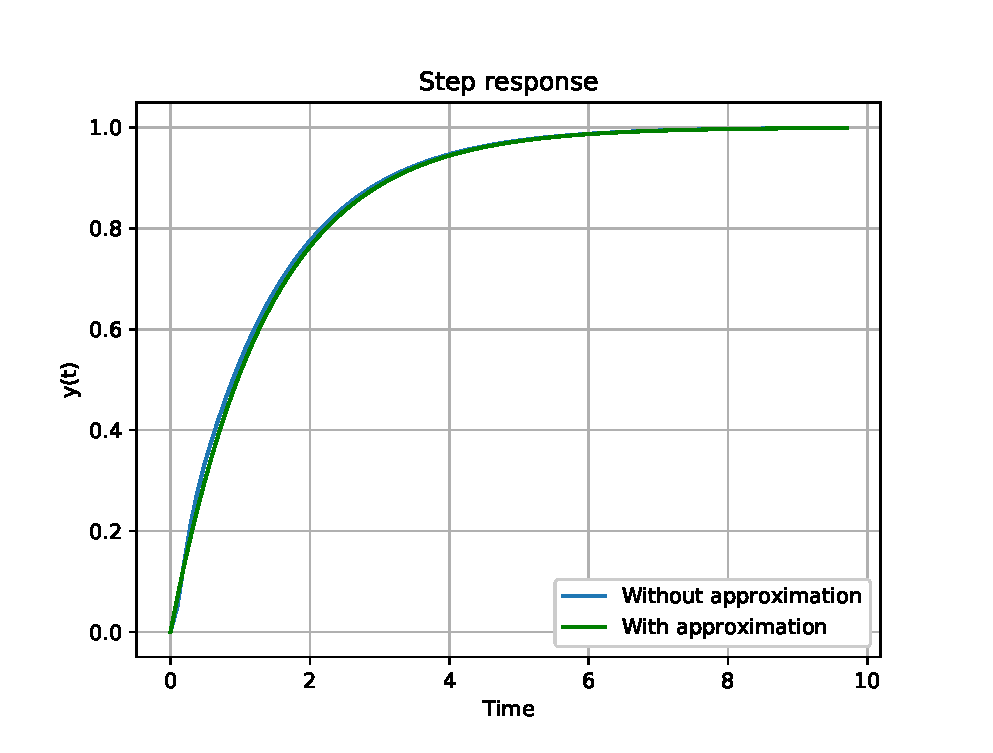
\includegraphics[width=\columnwidth]{./figs/ee18btech11047/ee18btech11047_4.eps}
\caption{}
\label{fig:ee18btech11047_4}
\end{figure}
\end{enumerate}
}
	\end{center}
\caption{}
\label{fig:ee18btech11047}
\end{figure}

\item Find the approximate transfer function for the open loop transfer function.
\begin{align}
G(s) &= \frac{50(s+3)(s+5)}{s(s+2)(s+4)(s+6)}
\end{align}
\solution Using equation\eqref{eq:ee18btech11047_ctf}
\begin{align}
T(s) &= \frac{50(s^{2}+8s+15)}{s^4+12s^3+94s^2+448s+750}
\end{align}
The following code gives the poles and zeros of the transfer function.
\begin{lstlisting}
codes/ee18btech11047/ee18btech11047_1.py
\end{lstlisting}
\begin{table}[!ht]
\centering
\begin{enumerate}[label=\thesubsection.\arabic*.,ref=\thesubsection.\theenumi]
\numberwithin{equation}{enumi}

\item Consider the following transfer functions as open-loop transfer functions in two different unity feedback(negative) systems.
\begin{align}
G(s) &= \frac{50(s+3)(s+5)}{s(s+2)(s+4)(s+6)}
\end{align}
\begin{align}
G(s) &= \frac{75(1+0.2s)}{s(s^{2}+16s+100)} 
\end{align}
Estimate transient response of these systems from their respective bode plots.\\
\solution 
\begin{enumerate}
\item  The dominant pole approximation is used to characterize higher order systems because it is difficult to characterize and analyse systems with order greater than 3.
\item Consider a transfer function.
\begin{align}
H(s) = K\frac{\alpha\beta}{(s+\alpha)(s+\beta)}
\end{align}
It has two poles $-\alpha$ and $-\beta $. If the magnitude of $\beta$ is very large compared to $\alpha$ (typically if $\frac{|\beta|}{|\alpha|}$ $>$ 5  ) we can approximate for the transfer function assuming $s$ is sufficiently small compared to $\beta$ as follows.
\begin{align}
H(s) = K_{2}\brak{\frac{1}{s+\alpha}}
\end{align}
Note that the value of $H(0)$ should be unchanged for the exact and approximate transfer functions.This is necessary to ensure that the final value of the step response is unchanged.
\begin{align}
\lim_{t\to\infty} y(t) &= \lim_{s\to 0} sY(s)
\end{align}
\begin{align}
\lim_{t\to\infty} y(t) &= \lim_{s\to 0} sU(s)H(s) = H(0)
\end{align}
In order to acheive this we adjust the gain value of the approximated transfer function by equating $H(0)$ values.
\begin{align}
\implies H(s) = K\frac{\alpha}{(s+\alpha)}
\end{align}
\item In terms of poles, the pole closer to the origin is considered as the dominating pole.As considered above,the magnitude of $\alpha$ is small therefore the time constant $\frac{1}{\alpha}$ will be high and reaches equilibrium slowly and vice versa in case of  $\beta$.Therefore,this approximation assumes that the slowest part of the system dominates the response.The faster parts of the system are ignored.
\item Complex poles along with real poles : In this case the dominant pole(s) can be determined by comparing only the real parts.If the real part of the complex conjugate poles is greater in magnitude than the real pole, the two complex conjugate poles the dominant poles.
\item If the transfer function has zeros along with poles,we have to consider the fact that pole and zero cancel out each other if their respective magnitudes are comparable.
\end{enumerate}
\item Find the closed loop transfer function of a negative unity feedback system given open loop transfer function $G(s)$ .\\
\solution 
\begin{align}
\label{eq:ee18btech11047_ctf}
T(s) &= \frac{G(s)}{1+G(s)}
\end{align}
\begin{figure}[!ht]
	\begin{center}
		\resizebox{\columnwidth}{!}{\input{./figs/ee18btech11047/ee18btech11047.tex}}
	\end{center}
\caption{}
\label{fig:ee18btech11047}
\end{figure}

\item Find the approximate transfer function for the open loop transfer function.
\begin{align}
G(s) &= \frac{50(s+3)(s+5)}{s(s+2)(s+4)(s+6)}
\end{align}
\solution Using equation\eqref{eq:ee18btech11047_ctf}
\begin{align}
T(s) &= \frac{50(s^{2}+8s+15)}{s^4+12s^3+94s^2+448s+750}
\end{align}
The following code gives the poles and zeros of the transfer function.
\begin{lstlisting}
codes/ee18btech11047/ee18btech11047_1.py
\end{lstlisting}
\begin{table}[!ht]
\centering
\input{./tables/ee18btech11047/ee18btech11047.tex}
\caption{}
\label{table:ee18btech11047}
\end{table}
The real poles \brak{p_{1},p_{2}} and zeros \brak{z_{1},z_{2}} cancel out each other as mentioned above.So, we are left with the two conjugate poles.The approximated transfer function is 
\begin{align}
T_{1}(s) &= \frac{K_{1}}{(s-p_{3})(s-p_{4})}
\end{align}
\begin{align}
T(0) &= T_{1}(0)
\end{align}
\begin{align}
\implies K_{1} &= p_{3}p_{4}
\end{align}
\begin{align}
T_{1}(s) &= \frac{47.09}{s^{2}+3.74s+47.09}
\end{align}

\item Estimate the transient response of the obtained second order system using the respective bode plot.\\
\solution The following code generates the bode plot for open loop transfer function.
\begin{lstlisting}
codes/ee18btech11047/ee18btech11047_2.py
\end{lstlisting}
\begin{figure}[!ht]
\centering
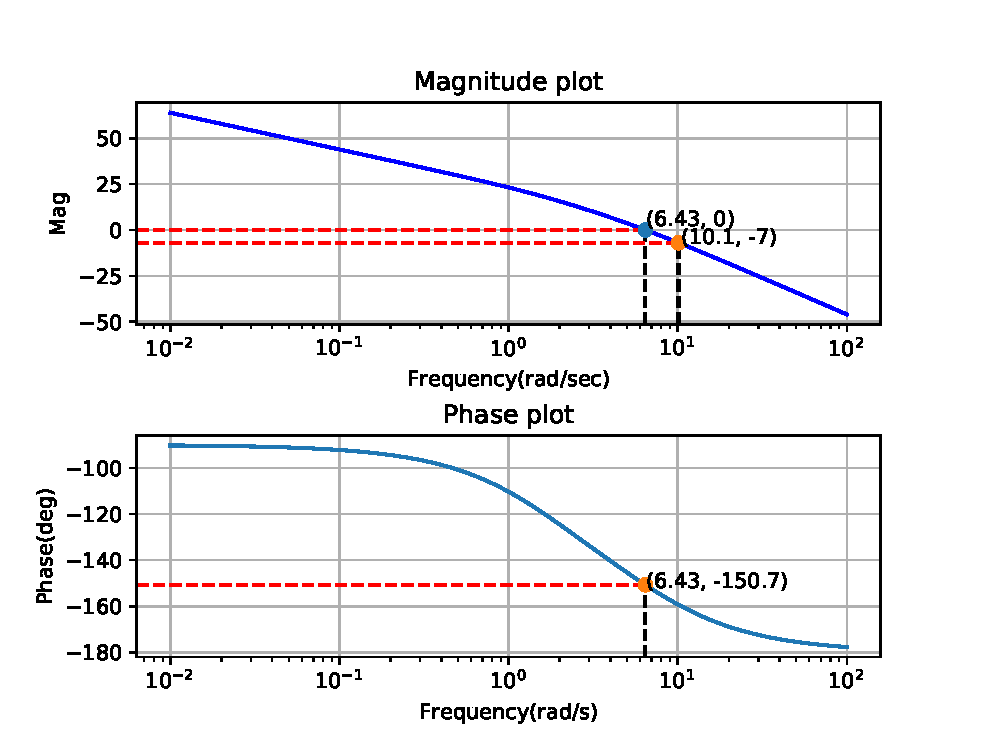
\includegraphics[width=\columnwidth]{./figs/ee18btech11047/ee18btech11047_2.eps}
\caption{1}
\label{fig:ee18btech11047_2}
\end{figure}
The phase margin is 
\begin{align}
\phi_{M} &= 180\degree-150.7\degree \implies \phi_{M} = 29.3\degree \label{eq:ee18btech11047_ph}
\end{align}
The closed-loop bandwith, $\omega_{BW}$(-3 dB frequency), equals the frequency at which the open-loop magnitude response is around -7 dB.
\begin{align}
\omega_{BW} = 10.1  rad/sec \label{eq:ee18btech11047_bw}
\end{align}
\textbf{Damping ratio:}
Substitute $\phi_{M}$ value from equation \eqref{eq:ee18btech11047_ph}
\begin{align}
\phi_{M} &= {tan}^{-1}\brak{\frac{2\zeta}{\sqrt{-2\zeta^{2}+\sqrt{1+4\zeta^{2}}}}}
\end{align}
\begin{align}
\implies \zeta &= 0.34
\end{align}
\textbf{Settling time:}
Substitute $\omega_{BW}$ value from equation\eqref{eq:ee18btech11047_bw} and $\zeta$
\begin{align}
T_{s}&= \frac{4}{\omega_{BW}\zeta}\sqrt{(1-2\zeta^2)+\sqrt{4\zeta^4-4\zeta^2+2}}
\end{align}
\begin{align}
\implies T_{s} &= 1.65 sec
\end{align}
\textbf{Peak time:}
\begin{align}
T_{p} &= \frac{\pi\zeta T_{s}}{4\sqrt{1-\zeta^2}}
\end{align}
\begin{align}
\implies T_{p} &= 0.325 sec
\end{align}
\textbf{Percent overshoot:}
\begin{align}
\% OS&=100e^{-(\frac{\zeta\pi}{\sqrt{1-\zeta^2}})}
\end{align}
\begin{align}
\implies \% OS &= 35.1 \%
\end{align}
Note that the answers will be approximate due to the dominant pole approximation.The following code generates the step response of the system.
\begin{lstlisting}
codes/ee18btech11047/ee18btech11047_3.py
\end{lstlisting}
\begin{figure}[!ht]
\centering
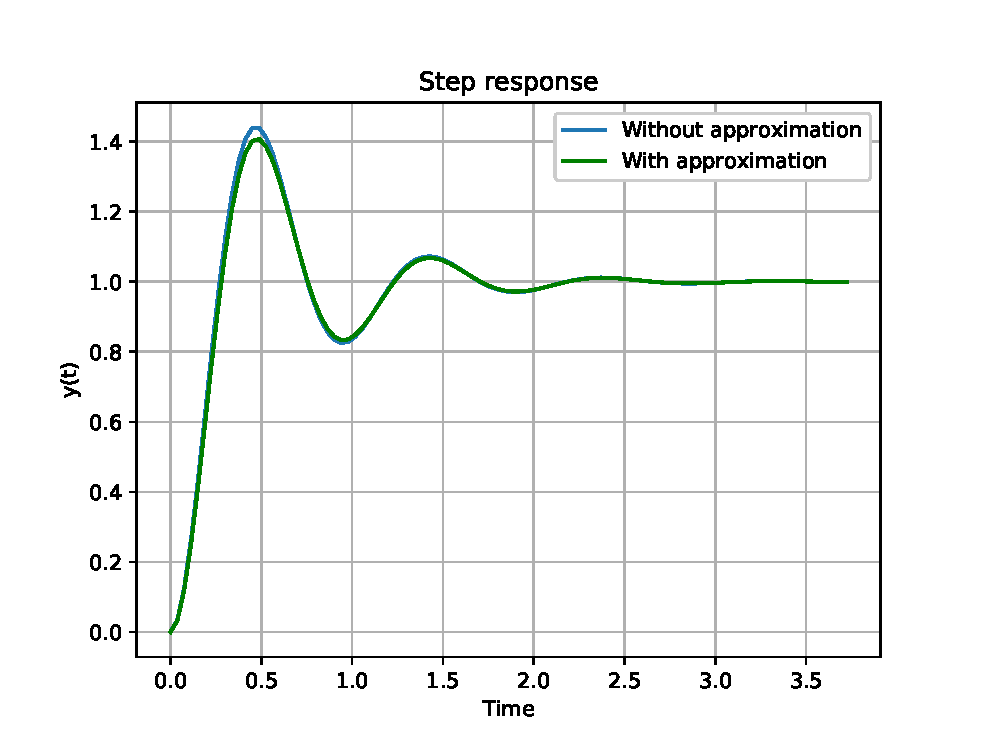
\includegraphics[width=\columnwidth]{./figs/ee18btech11047/ee18btech11047_3.eps}
\caption{2}
\label{fig:ee18btech11047_3}
\end{figure}
\item Find the approximate transfer function for the open loop transfer function
\begin{align}
G(s) &= \frac{75(1+0.2s)}{s(s^{2}+16s+100)}
\end{align}
\solution Using equation \eqref{eq:ee18btech11047_ctf}
\begin{align}
T(s) = \frac{75(1+0.2s)}{s^3 + 16s^2 + 115s +75} 
\end{align}
The following code gives the poles and zeros of the transfer function.
\begin{lstlisting}
codes/ee18btech11047/ee18btech11047_4.py
\end{lstlisting}
\begin{table}[!ht]
\centering
\input{./tables/ee18btech11047/ee18btech11047_2.tex}
\caption{}
\label{table:ee18btech11047_2}
\end{table}
The real part of the complex conjugate poles is comparable with the zero $z_{1}$ of the transfer function.So,they cancel out each other.The approximated transfer function is of first order.
\begin{align}
T_{2}(s) &= \frac{K_{2}}{(s-p_{1})}
\end{align}
\begin{align}
T(0) &= T_{2}(s)
\end{align}
\begin{align}
\implies K_{2} &= p_{1}
\end{align}
\begin{align}
T_{2}(s) &= \frac{0.72}{s+0.72}
\end{align}
\item Estimate the transient response of the obtained first order system.\\
\solution
\textbf{Time constant:}
The time constant is the time taken by the step response to rise to 63\% of it's final value.
\begin{align}
T &= \frac{1}{|pole|}
\end{align}
\begin{align}
T &= \frac{1}{0.72} = 1.388 sec
\end{align}
\textbf{Rise time:}
Rise time is the time for the waveform to go from 0.1 to 0.9 of it's final value.
\begin{align}
T_{r} &= \frac{2.2}{|pole|}
\end{align}
\begin{align}
T_{r} &= \frac{2.2}{0.72} = 3.05 sec
\end{align}
\textbf{Settling time:}
Settling time is defined as the time for the response to reach and stay within, 2\% of its final value.
\begin{align}
T_{s} &= \frac{4}{|pole|}
\end{align}
\begin{align}
T_{s} &= \frac{4}{0.72}=5.55 sec
\end{align}
The following code plots the step response of the system.
\begin{lstlisting}
codes/ee18btech11047/ee18btech11047_5.py
\end{lstlisting}
\begin{figure}[!ht]
\centering
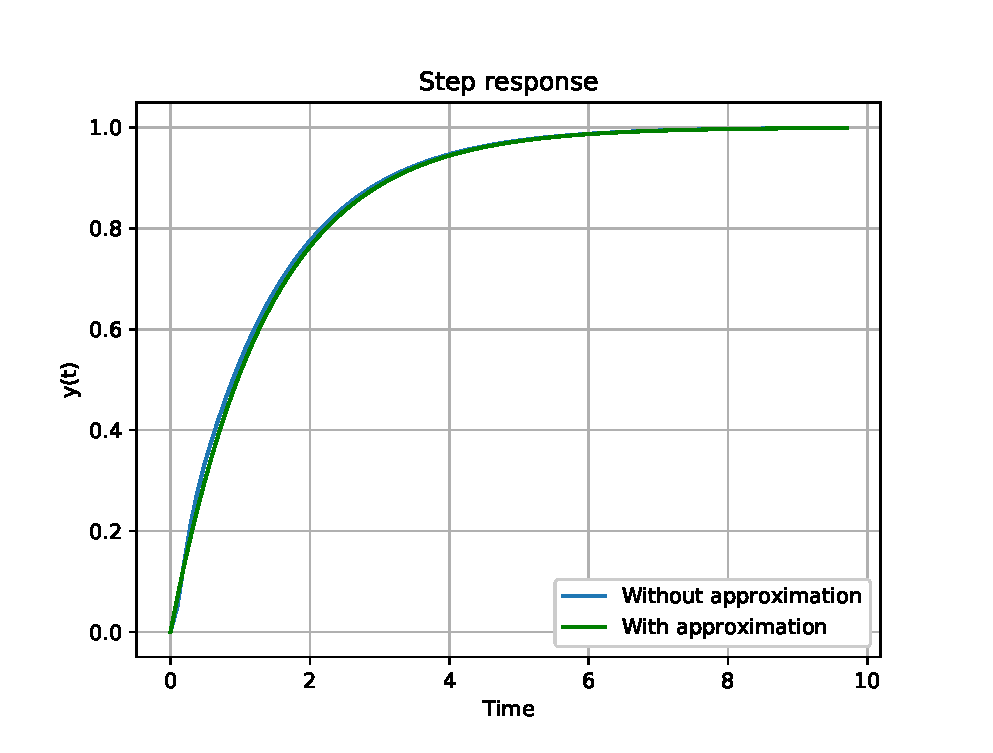
\includegraphics[width=\columnwidth]{./figs/ee18btech11047/ee18btech11047_4.eps}
\caption{}
\label{fig:ee18btech11047_4}
\end{figure}
\end{enumerate}

\caption{}
\label{table:ee18btech11047}
\end{table}
The real poles \brak{p_{1},p_{2}} and zeros \brak{z_{1},z_{2}} cancel out each other as mentioned above.So, we are left with the two conjugate poles.The approximated transfer function is 
\begin{align}
T_{1}(s) &= \frac{K_{1}}{(s-p_{3})(s-p_{4})}
\end{align}
\begin{align}
T(0) &= T_{1}(0)
\end{align}
\begin{align}
\implies K_{1} &= p_{3}p_{4}
\end{align}
\begin{align}
T_{1}(s) &= \frac{47.09}{s^{2}+3.74s+47.09}
\end{align}

\item Estimate the transient response of the obtained second order system using the respective bode plot.\\
\solution The following code generates the bode plot for open loop transfer function.
\begin{lstlisting}
codes/ee18btech11047/ee18btech11047_2.py
\end{lstlisting}
\begin{figure}[!ht]
\centering
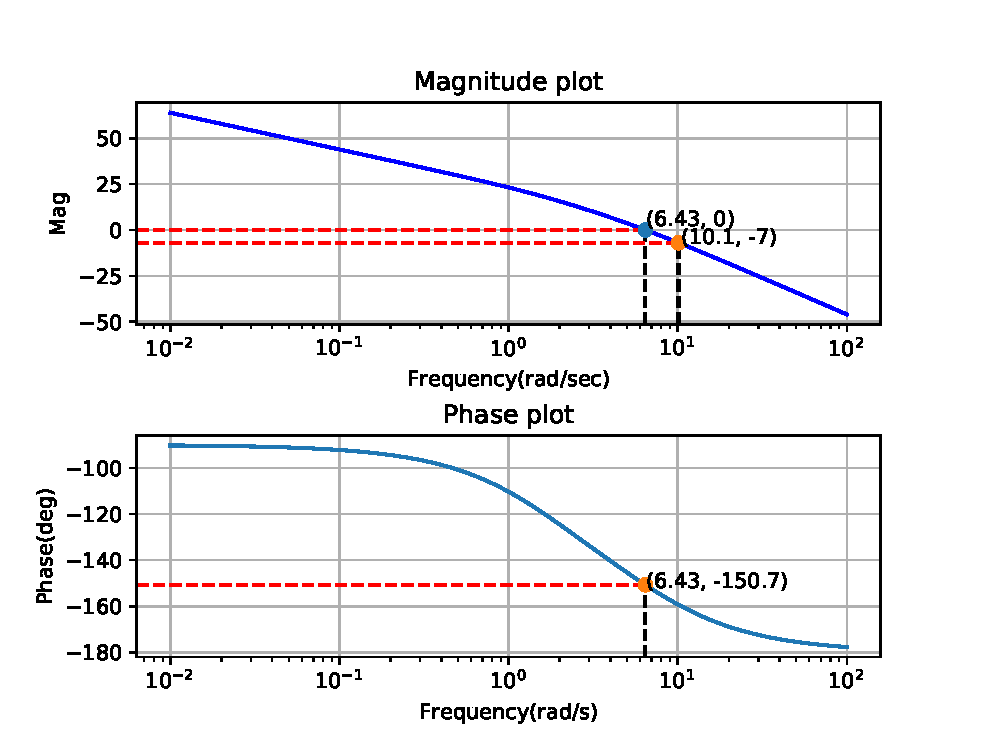
\includegraphics[width=\columnwidth]{./figs/ee18btech11047/ee18btech11047_2.eps}
\caption{1}
\label{fig:ee18btech11047_2}
\end{figure}
The phase margin is 
\begin{align}
\phi_{M} &= 180\degree-150.7\degree \implies \phi_{M} = 29.3\degree \label{eq:ee18btech11047_ph}
\end{align}
The closed-loop bandwith, $\omega_{BW}$(-3 dB frequency), equals the frequency at which the open-loop magnitude response is around -7 dB.
\begin{align}
\omega_{BW} = 10.1  rad/sec \label{eq:ee18btech11047_bw}
\end{align}
\textbf{Damping ratio:}
Substitute $\phi_{M}$ value from equation \eqref{eq:ee18btech11047_ph}
\begin{align}
\phi_{M} &= {tan}^{-1}\brak{\frac{2\zeta}{\sqrt{-2\zeta^{2}+\sqrt{1+4\zeta^{2}}}}}
\end{align}
\begin{align}
\implies \zeta &= 0.34
\end{align}
\textbf{Settling time:}
Substitute $\omega_{BW}$ value from equation\eqref{eq:ee18btech11047_bw} and $\zeta$
\begin{align}
T_{s}&= \frac{4}{\omega_{BW}\zeta}\sqrt{(1-2\zeta^2)+\sqrt{4\zeta^4-4\zeta^2+2}}
\end{align}
\begin{align}
\implies T_{s} &= 1.65 sec
\end{align}
\textbf{Peak time:}
\begin{align}
T_{p} &= \frac{\pi\zeta T_{s}}{4\sqrt{1-\zeta^2}}
\end{align}
\begin{align}
\implies T_{p} &= 0.325 sec
\end{align}
\textbf{Percent overshoot:}
\begin{align}
\% OS&=100e^{-(\frac{\zeta\pi}{\sqrt{1-\zeta^2}})}
\end{align}
\begin{align}
\implies \% OS &= 35.1 \%
\end{align}
Note that the answers will be approximate due to the dominant pole approximation.The following code generates the step response of the system.
\begin{lstlisting}
codes/ee18btech11047/ee18btech11047_3.py
\end{lstlisting}
\begin{figure}[!ht]
\centering
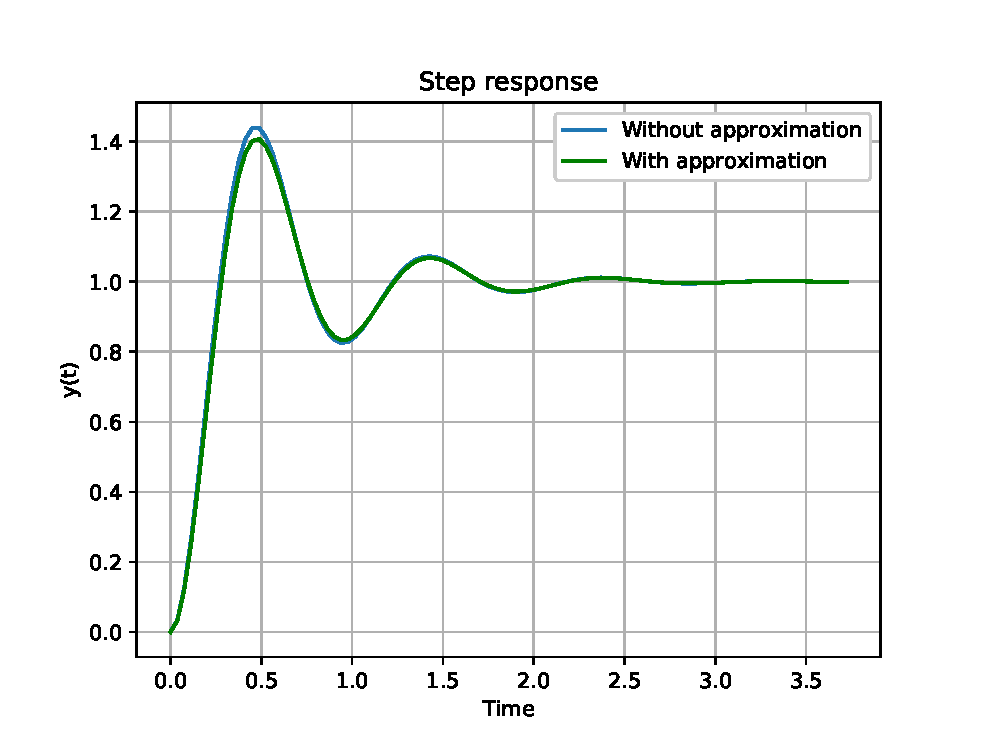
\includegraphics[width=\columnwidth]{./figs/ee18btech11047/ee18btech11047_3.eps}
\caption{2}
\label{fig:ee18btech11047_3}
\end{figure}
\item Find the approximate transfer function for the open loop transfer function
\begin{align}
G(s) &= \frac{75(1+0.2s)}{s(s^{2}+16s+100)}
\end{align}
\solution Using equation \eqref{eq:ee18btech11047_ctf}
\begin{align}
T(s) = \frac{75(1+0.2s)}{s^3 + 16s^2 + 115s +75} 
\end{align}
The following code gives the poles and zeros of the transfer function.
\begin{lstlisting}
codes/ee18btech11047/ee18btech11047_4.py
\end{lstlisting}
\begin{table}[!ht]
\centering
%%%%%%%%%%%%%%%%%%%%%%%%%%%%%%%%%%%%%%%%%%%%%%%%%%%%%%%%%%%%%%%%%%%%%%
%%                                                                  %%
%%  This is the header of a LaTeX2e file exported from Gnumeric.    %%
%%                                                                  %%
%%  This file can be compiled as it stands or included in another   %%
%%  LaTeX document. The table is based on the longtable package so  %%
%%  the longtable options (headers, footers...) can be set in the   %%
%%  preamble section below (see PRAMBLE).                           %%
%%                                                                  %%
%%  To include the file in another, the following two lines must be %%
%%  in the including file:                                          %%
%%        \def\inputGnumericTable{}                                 %%
%%  at the beginning of the file and:                               %%
%%        \input{name-of-this-file.tex}                             %%
%%  where the table is to be placed. Note also that the including   %%
%%  file must use the following packages for the table to be        %%
%%  rendered correctly:                                             %%
%%    \usepackage[latin1]{inputenc}                                 %%
%%    \usepackage{color}                                            %%
%%    \usepackage{array}                                            %%
%%    \usepackage{longtable}                                        %%
%%    \usepackage{calc}                                             %%
%%    \usepackage{multirow}                                         %%
%%    \usepackage{hhline}                                           %%
%%    \usepackage{ifthen}                                           %%
%%  optionally (for landscape tables embedded in another document): %%
%%    \usepackage{lscape}                                           %%
%%                                                                  %%
%%%%%%%%%%%%%%%%%%%%%%%%%%%%%%%%%%%%%%%%%%%%%%%%%%%%%%%%%%%%%%%%%%%%%%



%%  This section checks if we are begin input into another file or  %%
%%  the file will be compiled alone. First use a macro taken from   %%
%%  the TeXbook ex 7.7 (suggestion of Han-Wen Nienhuys).            %%
\def\ifundefined#1{\expandafter\ifx\csname#1\endcsname\relax}


%%  Check for the \def token for inputed files. If it is not        %%
%%  defined, the file will be processed as a standalone and the     %%
%%  preamble will be used.                                          %%
\ifundefined{inputGnumericTable}

%%  We must be able to close or not the document at the end.        %%
	\def\gnumericTableEnd{\end{document}}


%%%%%%%%%%%%%%%%%%%%%%%%%%%%%%%%%%%%%%%%%%%%%%%%%%%%%%%%%%%%%%%%%%%%%%
%%                                                                  %%
%%  This is the PREAMBLE. Change these values to get the right      %%
%%  paper size and other niceties.                                  %%
%%                                                                  %%
%%%%%%%%%%%%%%%%%%%%%%%%%%%%%%%%%%%%%%%%%%%%%%%%%%%%%%%%%%%%%%%%%%%%%%

	\documentclass[12pt%
			  %,landscape%
                    ]{report}
       \usepackage[latin1]{inputenc}
       \usepackage{fullpage}
       \usepackage{color}
       \usepackage{array}
       \usepackage{longtable}
       \usepackage{calc}
       \usepackage{multirow}
       \usepackage{hhline}
       \usepackage{ifthen}

	\begin{document}


%%  End of the preamble for the standalone. The next section is for %%
%%  documents which are included into other LaTeX2e files.          %%
\else

%%  We are not a stand alone document. For a regular table, we will %%
%%  have no preamble and only define the closing to mean nothing.   %%
    \def\gnumericTableEnd{}

%%  If we want landscape mode in an embedded document, comment out  %%
%%  the line above and uncomment the two below. The table will      %%
%%  begin on a new page and run in landscape mode.                  %%
%       \def\gnumericTableEnd{\end{landscape}}
%       \begin{landscape}


%%  End of the else clause for this file being \input.              %%
\fi

%%%%%%%%%%%%%%%%%%%%%%%%%%%%%%%%%%%%%%%%%%%%%%%%%%%%%%%%%%%%%%%%%%%%%%
%%                                                                  %%
%%  The rest is the gnumeric table, except for the closing          %%
%%  statement. Changes below will alter the table's appearance.     %%
%%                                                                  %%
%%%%%%%%%%%%%%%%%%%%%%%%%%%%%%%%%%%%%%%%%%%%%%%%%%%%%%%%%%%%%%%%%%%%%%

\providecommand{\gnumericmathit}[1]{#1} 
%%  Uncomment the next line if you would like your numbers to be in %%
%%  italics if they are italizised in the gnumeric table.           %%
%\renewcommand{\gnumericmathit}[1]{\mathit{#1}}
\providecommand{\gnumericPB}[1]%
{\let\gnumericTemp=\\#1\let\\=\gnumericTemp\hspace{0pt}}
 \ifundefined{gnumericTableWidthDefined}
        \newlength{\gnumericTableWidth}
        \newlength{\gnumericTableWidthComplete}
        \newlength{\gnumericMultiRowLength}
        \global\def\gnumericTableWidthDefined{}
 \fi
%% The following setting protects this code from babel shorthands.  %%
 \ifthenelse{\isundefined{\languageshorthands}}{}{\languageshorthands{english}}
%%  The default table format retains the relative column widths of  %%
%%  gnumeric. They can easily be changed to c, r or l. In that case %%
%%  you may want to comment out the next line and uncomment the one %%
%%  thereafter                                                      %%
\providecommand\gnumbox{\makebox[0pt]}
%%\providecommand\gnumbox[1][]{\makebox}

%% to adjust positions in multirow situations                       %%
\setlength{\bigstrutjot}{\jot}
\setlength{\extrarowheight}{\doublerulesep}

%%  The \setlongtables command keeps column widths the same across  %%
%%  pages. Simply comment out next line for varying column widths.  %%
\setlongtables

\setlength\gnumericTableWidth{%
	53pt+%
	93pt+%
0pt}
\def\gumericNumCols{2}
\setlength\gnumericTableWidthComplete{\gnumericTableWidth+%
         \tabcolsep*\gumericNumCols*2+\arrayrulewidth*\gumericNumCols}
\ifthenelse{\lengthtest{\gnumericTableWidthComplete > \linewidth}}%
         {\def\gnumericScale{\ratio{\linewidth-%
                        \tabcolsep*\gumericNumCols*2-%
                        \arrayrulewidth*\gumericNumCols}%
{\gnumericTableWidth}}}%
{\def\gnumericScale{1}}

%%%%%%%%%%%%%%%%%%%%%%%%%%%%%%%%%%%%%%%%%%%%%%%%%%%%%%%%%%%%%%%%%%%%%%
%%                                                                  %%
%% The following are the widths of the various columns. We are      %%
%% defining them here because then they are easier to change.       %%
%% Depending on the cell formats we may use them more than once.    %%
%%                                                                  %%
%%%%%%%%%%%%%%%%%%%%%%%%%%%%%%%%%%%%%%%%%%%%%%%%%%%%%%%%%%%%%%%%%%%%%%

\ifthenelse{\isundefined{\gnumericColA}}{\newlength{\gnumericColA}}{}\settowidth{\gnumericColA}{\begin{tabular}{@{}p{90pt*\gnumericScale}@{}}x\end{tabular}}
\ifthenelse{\isundefined{\gnumericColB}}{\newlength{\gnumericColB}}{}\settowidth{\gnumericColB}{\begin{tabular}{@{}p{53pt*\gnumericScale}@{}}x\end{tabular}}

\begin{tabular}[c]{%
	b{\gnumericColA}%
	b{\gnumericColB}%
	}

%%%%%%%%%%%%%%%%%%%%%%%%%%%%%%%%%%%%%%%%%%%%%%%%%%%%%%%%%%%%%%%%%%%%%%
%%  The longtable options. (Caption, headers... see Goosens, p.124) %%
%	\caption{The Table Caption.}             \\	%
% \hline	% Across the top of the table.
%%  The rest of these options are table rows which are placed on    %%
%%  the first, last or every page. Use \multicolumn if you want.    %%

%%  Header for the first page.                                      %%
%	\multicolumn{2}{c}{The First Header} \\ \hline 
%	\multicolumn{1}{c}{colTag}	%Column 1
%	&\multicolumn{1}{c}{colTag}	\\ \hline %Last column
%	\endfirsthead

%%  The running header definition.                                  %%
%	\hline
%	\multicolumn{2}{l}{\ldots\small\slshape continued} \\ \hline
%	\multicolumn{1}{c}{colTag}	%Column 1
%	&\multicolumn{1}{c}{colTag}	\\ \hline %Last column
%	\endhead

%%  The running footer definition.                                  %%
%	\hline
%	\multicolumn{2}{r}{\small\slshape continued\ldots} \\
%	\endfoot

%%  The ending footer definition.                                   %%
%	\multicolumn{2}{c}{That's all folks} \\ \hline 
%	\endlastfoot
%%%%%%%%%%%%%%%%%%%%%%%%%%%%%%%%%%%%%%%%%%%%%%%%%%%%%%%%%%%%%%%%%%%%%%

\hhline{|-|-}
	 \multicolumn{1}{|p{\gnumericColA}|}%
	{\gnumericPB{\centering}\gnumbox{\textbf{Poles}}}
	&\multicolumn{1}{p{\gnumericColB}|}%
	{\gnumericPB{\centering}\gnumbox{\textbf{Zeros}}}
\\
\hhline{|--|}
	 \multicolumn{1}{|p{\gnumericColA}|}%
	{\gnumericPB{\centering}\gnumbox{$p_{1}=-0.72$}}
	&\multicolumn{1}{p{\gnumericColB}|}%
	{$z_{1}=-5$}
\\
\hhline{|--|}
	 \multicolumn{1}{|p{\gnumericColA}|}%
	{\gnumericPB{\centering}\gnumbox{$p_{2}=-7.64+6.75j$}}
	&\multicolumn{1}{p{\gnumericColB}|}%
	{}
\\
\hhline{|--|}
	 \multicolumn{1}{|p{\gnumericColA}|}%
	{\gnumericPB{\centering}\gnumbox{$p_{3}=-7.63-6.75j$}}
	&\multicolumn{1}{p{\gnumericColB}|}%
	{}
\\
\hhline{|-|-|}
\end{tabular}

\ifthenelse{\isundefined{\languageshorthands}}{}{\languageshorthands{\languagename}}
\gnumericTableEnd

\caption{}
\label{table:ee18btech11047_2}
\end{table}
The real part of the complex conjugate poles is comparable with the zero $z_{1}$ of the transfer function.So,they cancel out each other.The approximated transfer function is of first order.
\begin{align}
T_{2}(s) &= \frac{K_{2}}{(s-p_{1})}
\end{align}
\begin{align}
T(0) &= T_{2}(s)
\end{align}
\begin{align}
\implies K_{2} &= p_{1}
\end{align}
\begin{align}
T_{2}(s) &= \frac{0.72}{s+0.72}
\end{align}
\item Estimate the transient response of the obtained first order system.\\
\solution
\textbf{Time constant:}
The time constant is the time taken by the step response to rise to 63\% of it's final value.
\begin{align}
T &= \frac{1}{|pole|}
\end{align}
\begin{align}
T &= \frac{1}{0.72} = 1.388 sec
\end{align}
\textbf{Rise time:}
Rise time is the time for the waveform to go from 0.1 to 0.9 of it's final value.
\begin{align}
T_{r} &= \frac{2.2}{|pole|}
\end{align}
\begin{align}
T_{r} &= \frac{2.2}{0.72} = 3.05 sec
\end{align}
\textbf{Settling time:}
Settling time is defined as the time for the response to reach and stay within, 2\% of its final value.
\begin{align}
T_{s} &= \frac{4}{|pole|}
\end{align}
\begin{align}
T_{s} &= \frac{4}{0.72}=5.55 sec
\end{align}
The following code plots the step response of the system.
\begin{lstlisting}
codes/ee18btech11047/ee18btech11047_5.py
\end{lstlisting}
\begin{figure}[!ht]
\centering
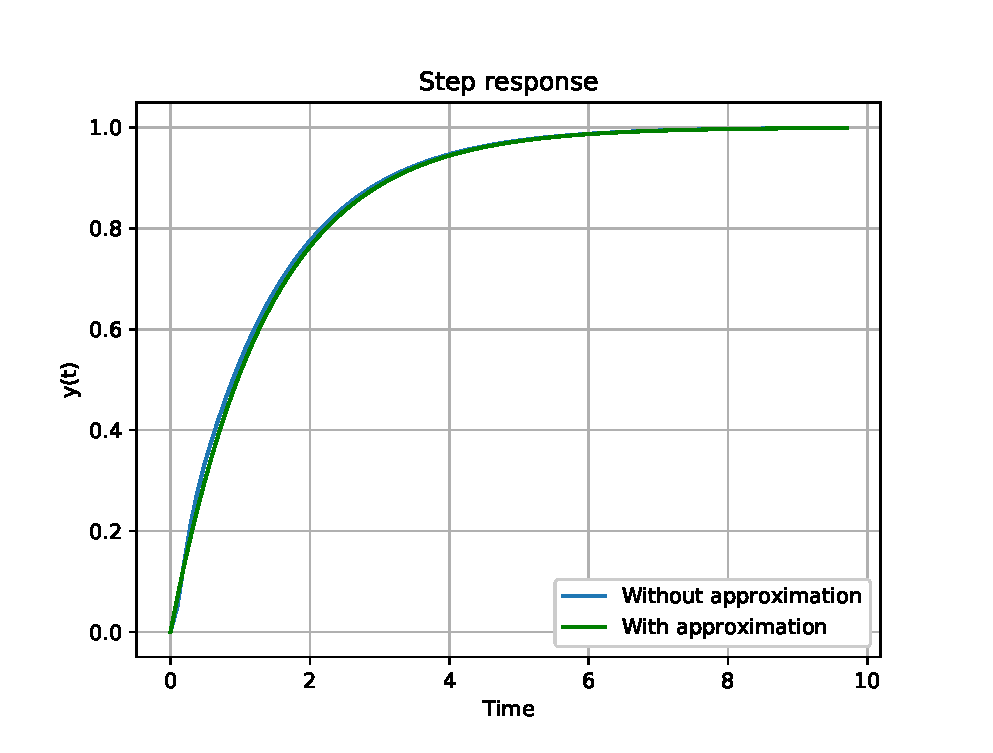
\includegraphics[width=\columnwidth]{./figs/ee18btech11047/ee18btech11047_4.eps}
\caption{}
\label{fig:ee18btech11047_4}
\end{figure}
\end{enumerate}

\caption{}
\label{table:ee18btech11047}
\end{table}
The real poles \brak{p_{1},p_{2}} and zeros \brak{z_{1},z_{2}} cancel out each other as mentioned above.So, we are left with the two conjugate poles.The approximated transfer function is 
\begin{align}
T_{1}(s) &= \frac{K_{1}}{(s-p_{3})(s-p_{4})}
\end{align}
\begin{align}
T(0) &= T_{1}(0)
\end{align}
\begin{align}
\implies K_{1} &= p_{3}p_{4}
\end{align}
\begin{align}
T_{1}(s) &= \frac{47.09}{s^{2}+3.74s+47.09}
\end{align}

\item Estimate the transient response of the obtained second order system using the respective bode plot.\\
\solution The following code generates the bode plot for open loop transfer function.
\begin{lstlisting}
codes/ee18btech11047/ee18btech11047_2.py
\end{lstlisting}
\begin{figure}[!ht]
\centering
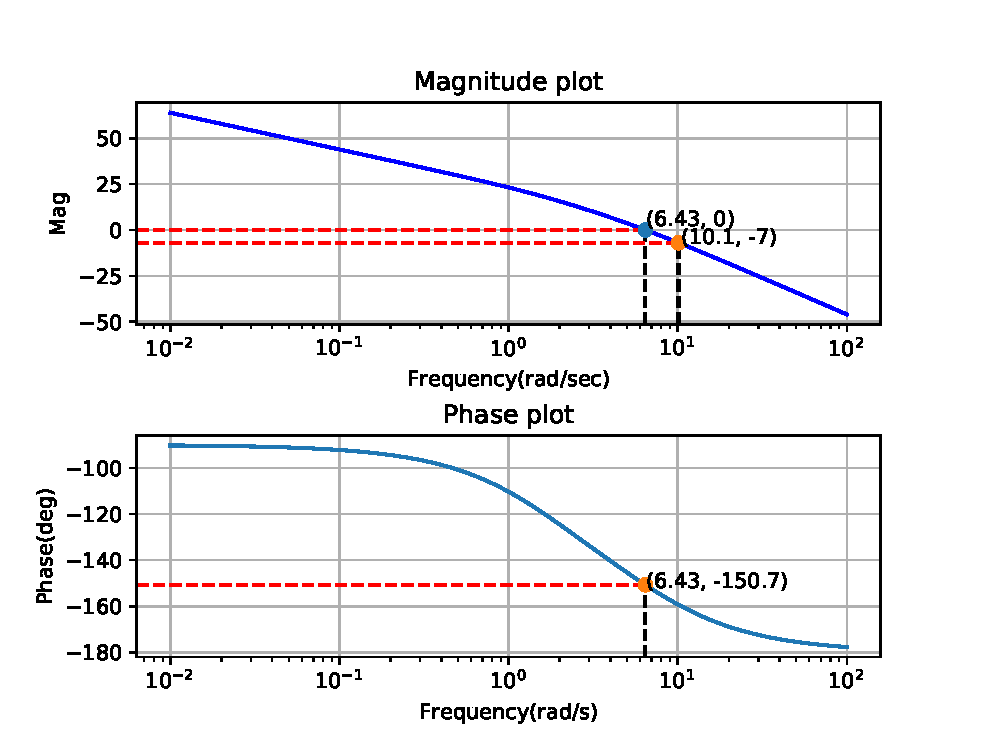
\includegraphics[width=\columnwidth]{./figs/ee18btech11047/ee18btech11047_2.eps}
\caption{1}
\label{fig:ee18btech11047_2}
\end{figure}
The phase margin is 
\begin{align}
\phi_{M} &= 180\degree-150.7\degree \implies \phi_{M} = 29.3\degree \label{eq:ee18btech11047_ph}
\end{align}
The closed-loop bandwith, $\omega_{BW}$(-3 dB frequency), equals the frequency at which the open-loop magnitude response is around -7 dB.
\begin{align}
\omega_{BW} = 10.1  rad/sec \label{eq:ee18btech11047_bw}
\end{align}
\textbf{Damping ratio:}
Substitute $\phi_{M}$ value from equation \eqref{eq:ee18btech11047_ph}
\begin{align}
\phi_{M} &= {tan}^{-1}\brak{\frac{2\zeta}{\sqrt{-2\zeta^{2}+\sqrt{1+4\zeta^{2}}}}}
\end{align}
\begin{align}
\implies \zeta &= 0.34
\end{align}
\textbf{Settling time:}
Substitute $\omega_{BW}$ value from equation\eqref{eq:ee18btech11047_bw} and $\zeta$
\begin{align}
T_{s}&= \frac{4}{\omega_{BW}\zeta}\sqrt{(1-2\zeta^2)+\sqrt{4\zeta^4-4\zeta^2+2}}
\end{align}
\begin{align}
\implies T_{s} &= 1.65 sec
\end{align}
\textbf{Peak time:}
\begin{align}
T_{p} &= \frac{\pi\zeta T_{s}}{4\sqrt{1-\zeta^2}}
\end{align}
\begin{align}
\implies T_{p} &= 0.325 sec
\end{align}
\textbf{Percent overshoot:}
\begin{align}
\% OS&=100e^{-(\frac{\zeta\pi}{\sqrt{1-\zeta^2}})}
\end{align}
\begin{align}
\implies \% OS &= 35.1 \%
\end{align}
Note that the answers will be approximate due to the dominant pole approximation.The following code generates the step response of the system.
\begin{lstlisting}
codes/ee18btech11047/ee18btech11047_3.py
\end{lstlisting}
\begin{figure}[!ht]
\centering
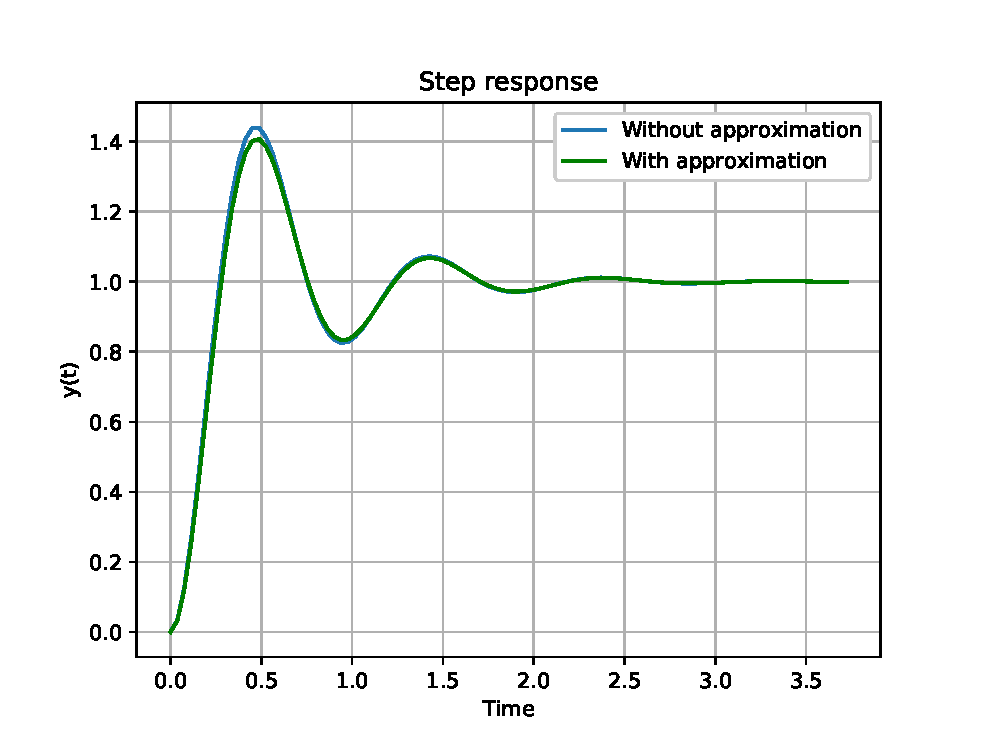
\includegraphics[width=\columnwidth]{./figs/ee18btech11047/ee18btech11047_3.eps}
\caption{2}
\label{fig:ee18btech11047_3}
\end{figure}
\item Find the approximate transfer function for the open loop transfer function
\begin{align}
G(s) &= \frac{75(1+0.2s)}{s(s^{2}+16s+100)}
\end{align}
\solution Using equation \eqref{eq:ee18btech11047_ctf}
\begin{align}
T(s) = \frac{75(1+0.2s)}{s^3 + 16s^2 + 115s +75} 
\end{align}
The following code gives the poles and zeros of the transfer function.
\begin{lstlisting}
codes/ee18btech11047/ee18btech11047_4.py
\end{lstlisting}
\begin{table}[!ht]
\centering
%%%%%%%%%%%%%%%%%%%%%%%%%%%%%%%%%%%%%%%%%%%%%%%%%%%%%%%%%%%%%%%%%%%%%%
%%                                                                  %%
%%  This is the header of a LaTeX2e file exported from Gnumeric.    %%
%%                                                                  %%
%%  This file can be compiled as it stands or included in another   %%
%%  LaTeX document. The table is based on the longtable package so  %%
%%  the longtable options (headers, footers...) can be set in the   %%
%%  preamble section below (see PRAMBLE).                           %%
%%                                                                  %%
%%  To include the file in another, the following two lines must be %%
%%  in the including file:                                          %%
%%        \def\inputGnumericTable{}                                 %%
%%  at the beginning of the file and:                               %%
%%        \input{name-of-this-file.tex}                             %%
%%  where the table is to be placed. Note also that the including   %%
%%  file must use the following packages for the table to be        %%
%%  rendered correctly:                                             %%
%%    \usepackage[latin1]{inputenc}                                 %%
%%    \usepackage{color}                                            %%
%%    \usepackage{array}                                            %%
%%    \usepackage{longtable}                                        %%
%%    \usepackage{calc}                                             %%
%%    \usepackage{multirow}                                         %%
%%    \usepackage{hhline}                                           %%
%%    \usepackage{ifthen}                                           %%
%%  optionally (for landscape tables embedded in another document): %%
%%    \usepackage{lscape}                                           %%
%%                                                                  %%
%%%%%%%%%%%%%%%%%%%%%%%%%%%%%%%%%%%%%%%%%%%%%%%%%%%%%%%%%%%%%%%%%%%%%%



%%  This section checks if we are begin input into another file or  %%
%%  the file will be compiled alone. First use a macro taken from   %%
%%  the TeXbook ex 7.7 (suggestion of Han-Wen Nienhuys).            %%
\def\ifundefined#1{\expandafter\ifx\csname#1\endcsname\relax}


%%  Check for the \def token for inputed files. If it is not        %%
%%  defined, the file will be processed as a standalone and the     %%
%%  preamble will be used.                                          %%
\ifundefined{inputGnumericTable}

%%  We must be able to close or not the document at the end.        %%
	\def\gnumericTableEnd{\end{document}}


%%%%%%%%%%%%%%%%%%%%%%%%%%%%%%%%%%%%%%%%%%%%%%%%%%%%%%%%%%%%%%%%%%%%%%
%%                                                                  %%
%%  This is the PREAMBLE. Change these values to get the right      %%
%%  paper size and other niceties.                                  %%
%%                                                                  %%
%%%%%%%%%%%%%%%%%%%%%%%%%%%%%%%%%%%%%%%%%%%%%%%%%%%%%%%%%%%%%%%%%%%%%%

	\documentclass[12pt%
			  %,landscape%
                    ]{report}
       \usepackage[latin1]{inputenc}
       \usepackage{fullpage}
       \usepackage{color}
       \usepackage{array}
       \usepackage{longtable}
       \usepackage{calc}
       \usepackage{multirow}
       \usepackage{hhline}
       \usepackage{ifthen}

	\begin{document}


%%  End of the preamble for the standalone. The next section is for %%
%%  documents which are included into other LaTeX2e files.          %%
\else

%%  We are not a stand alone document. For a regular table, we will %%
%%  have no preamble and only define the closing to mean nothing.   %%
    \def\gnumericTableEnd{}

%%  If we want landscape mode in an embedded document, comment out  %%
%%  the line above and uncomment the two below. The table will      %%
%%  begin on a new page and run in landscape mode.                  %%
%       \def\gnumericTableEnd{\end{landscape}}
%       \begin{landscape}


%%  End of the else clause for this file being \input.              %%
\fi

%%%%%%%%%%%%%%%%%%%%%%%%%%%%%%%%%%%%%%%%%%%%%%%%%%%%%%%%%%%%%%%%%%%%%%
%%                                                                  %%
%%  The rest is the gnumeric table, except for the closing          %%
%%  statement. Changes below will alter the table's appearance.     %%
%%                                                                  %%
%%%%%%%%%%%%%%%%%%%%%%%%%%%%%%%%%%%%%%%%%%%%%%%%%%%%%%%%%%%%%%%%%%%%%%

\providecommand{\gnumericmathit}[1]{#1} 
%%  Uncomment the next line if you would like your numbers to be in %%
%%  italics if they are italizised in the gnumeric table.           %%
%\renewcommand{\gnumericmathit}[1]{\mathit{#1}}
\providecommand{\gnumericPB}[1]%
{\let\gnumericTemp=\\#1\let\\=\gnumericTemp\hspace{0pt}}
 \ifundefined{gnumericTableWidthDefined}
        \newlength{\gnumericTableWidth}
        \newlength{\gnumericTableWidthComplete}
        \newlength{\gnumericMultiRowLength}
        \global\def\gnumericTableWidthDefined{}
 \fi
%% The following setting protects this code from babel shorthands.  %%
 \ifthenelse{\isundefined{\languageshorthands}}{}{\languageshorthands{english}}
%%  The default table format retains the relative column widths of  %%
%%  gnumeric. They can easily be changed to c, r or l. In that case %%
%%  you may want to comment out the next line and uncomment the one %%
%%  thereafter                                                      %%
\providecommand\gnumbox{\makebox[0pt]}
%%\providecommand\gnumbox[1][]{\makebox}

%% to adjust positions in multirow situations                       %%
\setlength{\bigstrutjot}{\jot}
\setlength{\extrarowheight}{\doublerulesep}

%%  The \setlongtables command keeps column widths the same across  %%
%%  pages. Simply comment out next line for varying column widths.  %%
\setlongtables

\setlength\gnumericTableWidth{%
	53pt+%
	93pt+%
0pt}
\def\gumericNumCols{2}
\setlength\gnumericTableWidthComplete{\gnumericTableWidth+%
         \tabcolsep*\gumericNumCols*2+\arrayrulewidth*\gumericNumCols}
\ifthenelse{\lengthtest{\gnumericTableWidthComplete > \linewidth}}%
         {\def\gnumericScale{\ratio{\linewidth-%
                        \tabcolsep*\gumericNumCols*2-%
                        \arrayrulewidth*\gumericNumCols}%
{\gnumericTableWidth}}}%
{\def\gnumericScale{1}}

%%%%%%%%%%%%%%%%%%%%%%%%%%%%%%%%%%%%%%%%%%%%%%%%%%%%%%%%%%%%%%%%%%%%%%
%%                                                                  %%
%% The following are the widths of the various columns. We are      %%
%% defining them here because then they are easier to change.       %%
%% Depending on the cell formats we may use them more than once.    %%
%%                                                                  %%
%%%%%%%%%%%%%%%%%%%%%%%%%%%%%%%%%%%%%%%%%%%%%%%%%%%%%%%%%%%%%%%%%%%%%%

\ifthenelse{\isundefined{\gnumericColA}}{\newlength{\gnumericColA}}{}\settowidth{\gnumericColA}{\begin{tabular}{@{}p{90pt*\gnumericScale}@{}}x\end{tabular}}
\ifthenelse{\isundefined{\gnumericColB}}{\newlength{\gnumericColB}}{}\settowidth{\gnumericColB}{\begin{tabular}{@{}p{53pt*\gnumericScale}@{}}x\end{tabular}}

\begin{tabular}[c]{%
	b{\gnumericColA}%
	b{\gnumericColB}%
	}

%%%%%%%%%%%%%%%%%%%%%%%%%%%%%%%%%%%%%%%%%%%%%%%%%%%%%%%%%%%%%%%%%%%%%%
%%  The longtable options. (Caption, headers... see Goosens, p.124) %%
%	\caption{The Table Caption.}             \\	%
% \hline	% Across the top of the table.
%%  The rest of these options are table rows which are placed on    %%
%%  the first, last or every page. Use \multicolumn if you want.    %%

%%  Header for the first page.                                      %%
%	\multicolumn{2}{c}{The First Header} \\ \hline 
%	\multicolumn{1}{c}{colTag}	%Column 1
%	&\multicolumn{1}{c}{colTag}	\\ \hline %Last column
%	\endfirsthead

%%  The running header definition.                                  %%
%	\hline
%	\multicolumn{2}{l}{\ldots\small\slshape continued} \\ \hline
%	\multicolumn{1}{c}{colTag}	%Column 1
%	&\multicolumn{1}{c}{colTag}	\\ \hline %Last column
%	\endhead

%%  The running footer definition.                                  %%
%	\hline
%	\multicolumn{2}{r}{\small\slshape continued\ldots} \\
%	\endfoot

%%  The ending footer definition.                                   %%
%	\multicolumn{2}{c}{That's all folks} \\ \hline 
%	\endlastfoot
%%%%%%%%%%%%%%%%%%%%%%%%%%%%%%%%%%%%%%%%%%%%%%%%%%%%%%%%%%%%%%%%%%%%%%

\hhline{|-|-}
	 \multicolumn{1}{|p{\gnumericColA}|}%
	{\gnumericPB{\centering}\gnumbox{\textbf{Poles}}}
	&\multicolumn{1}{p{\gnumericColB}|}%
	{\gnumericPB{\centering}\gnumbox{\textbf{Zeros}}}
\\
\hhline{|--|}
	 \multicolumn{1}{|p{\gnumericColA}|}%
	{\gnumericPB{\centering}\gnumbox{$p_{1}=-0.72$}}
	&\multicolumn{1}{p{\gnumericColB}|}%
	{$z_{1}=-5$}
\\
\hhline{|--|}
	 \multicolumn{1}{|p{\gnumericColA}|}%
	{\gnumericPB{\centering}\gnumbox{$p_{2}=-7.64+6.75j$}}
	&\multicolumn{1}{p{\gnumericColB}|}%
	{}
\\
\hhline{|--|}
	 \multicolumn{1}{|p{\gnumericColA}|}%
	{\gnumericPB{\centering}\gnumbox{$p_{3}=-7.63-6.75j$}}
	&\multicolumn{1}{p{\gnumericColB}|}%
	{}
\\
\hhline{|-|-|}
\end{tabular}

\ifthenelse{\isundefined{\languageshorthands}}{}{\languageshorthands{\languagename}}
\gnumericTableEnd

\caption{}
\label{table:ee18btech11047_2}
\end{table}
The real part of the complex conjugate poles is comparable with the zero $z_{1}$ of the transfer function.So,they cancel out each other.The approximated transfer function is of first order.
\begin{align}
T_{2}(s) &= \frac{K_{2}}{(s-p_{1})}
\end{align}
\begin{align}
T(0) &= T_{2}(s)
\end{align}
\begin{align}
\implies K_{2} &= p_{1}
\end{align}
\begin{align}
T_{2}(s) &= \frac{0.72}{s+0.72}
\end{align}
\item Estimate the transient response of the obtained first order system.\\
\solution
\textbf{Time constant:}
The time constant is the time taken by the step response to rise to 63\% of it's final value.
\begin{align}
T &= \frac{1}{|pole|}
\end{align}
\begin{align}
T &= \frac{1}{0.72} = 1.388 sec
\end{align}
\textbf{Rise time:}
Rise time is the time for the waveform to go from 0.1 to 0.9 of it's final value.
\begin{align}
T_{r} &= \frac{2.2}{|pole|}
\end{align}
\begin{align}
T_{r} &= \frac{2.2}{0.72} = 3.05 sec
\end{align}
\textbf{Settling time:}
Settling time is defined as the time for the response to reach and stay within, 2\% of its final value.
\begin{align}
T_{s} &= \frac{4}{|pole|}
\end{align}
\begin{align}
T_{s} &= \frac{4}{0.72}=5.55 sec
\end{align}
The following code plots the step response of the system.
\begin{lstlisting}
codes/ee18btech11047/ee18btech11047_5.py
\end{lstlisting}
\begin{figure}[!ht]
\centering
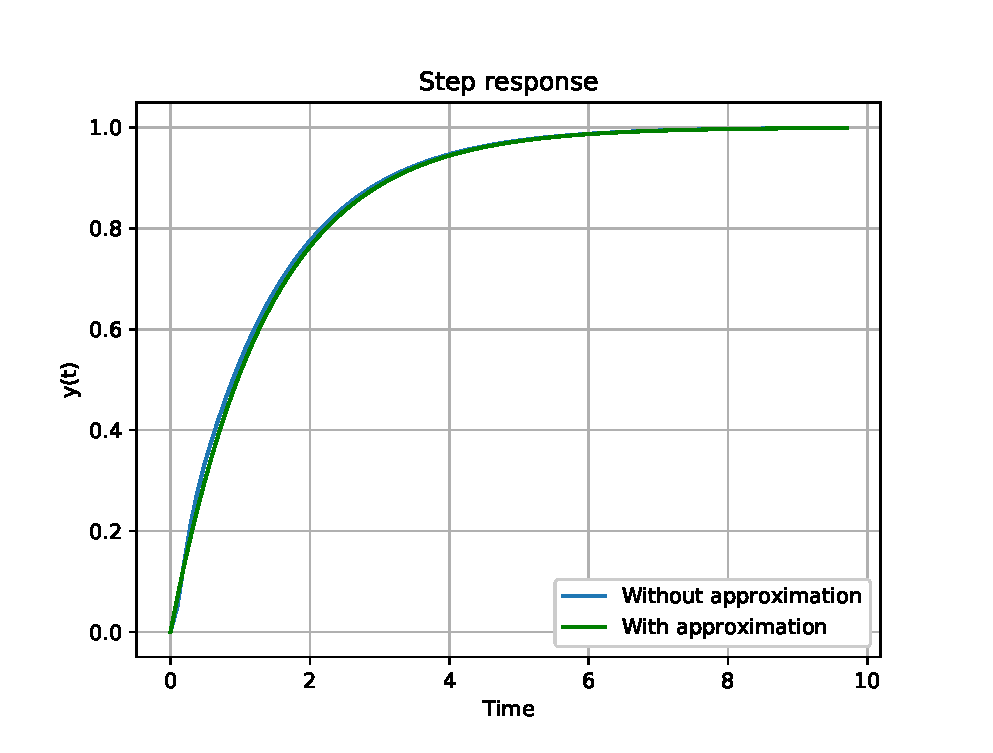
\includegraphics[width=\columnwidth]{./figs/ee18btech11047/ee18btech11047_4.eps}
\caption{}
\label{fig:ee18btech11047_4}
\end{figure}
\end{enumerate}

\end{document}
